% Created 2021-11-04 to 18:44
% Intended LaTeX compiler: pdflatex
\documentclass[12pt]{article}

%%%% settings when exporting code %%%% 

\usepackage{listings}
\lstdefinestyle{code-small}{
backgroundcolor=\color{white}, % background color for the code block
basicstyle=\ttfamily\small, % font used to display the code
commentstyle=\color[rgb]{0.5,0,0.5}, % color used to display comments in the code
keywordstyle=\color{black}, % color used to highlight certain words in the code
numberstyle=\ttfamily\tiny\color{gray}, % color used to display the line numbers
rulecolor=\color{black}, % color of the frame
stringstyle=\color[rgb]{0,.5,0},  % color used to display strings in the code
breakatwhitespace=false, % sets if automatic breaks should only happen at whitespace
breaklines=true, % sets automatic line breaking
columns=fullflexible,
frame=single, % adds a frame around the code (non,leftline,topline,bottomline,lines,single,shadowbox)
keepspaces=true, % % keeps spaces in text, useful for keeping indentation of code
literate={~}{$\sim$}{1}, % symbol properly display via latex
numbers=none, % where to put the line-numbers; possible values are (none, left, right)
numbersep=10pt, % how far the line-numbers are from the code
showspaces=false,
showstringspaces=false,
stepnumber=1, % the step between two line-numbers. If it's 1, each line will be numbered
tabsize=1,
xleftmargin=0cm,
emph={anova,apply,class,coef,colnames,colNames,colSums,dim,dcast,for,ggplot,head,if,ifelse,is.na,lapply,list.files,library,logLik,melt,plot,require,rowSums,sapply,setcolorder,setkey,str,summary,tapply},
aboveskip = \medskipamount, % define the space above displayed listings.
belowskip = \medskipamount, % define the space above displayed listings.
lineskip = 0pt} % specifies additional space between lines in listings
\lstset{style=code-small}
%%%% packages %%%%%

\usepackage[utf8]{inputenc}
\usepackage[T1]{fontenc}
\usepackage{lmodern}
\usepackage{textcomp}
\usepackage{color}
\usepackage{graphicx}
\usepackage{grffile}
\usepackage{wrapfig}
\usepackage{rotating}
\usepackage{longtable}
\usepackage{multirow}
\usepackage{multicol}
\usepackage{changes}
\usepackage{pdflscape}
\usepackage{geometry}
\usepackage[normalem]{ulem}
\usepackage{amssymb}
\usepackage{amsmath}
\usepackage{amsfonts}
\usepackage{dsfont}
\usepackage{array}
\usepackage{ifthen}
\usepackage{hyperref}
\usepackage{natbib}
\RequirePackage{setspace} % to modify the space between lines - incompatible with footnote in beamer
\renewcommand{\baselinestretch}{1.1}
\geometry{a4paper, left=10mm, right=10mm, top=10mm}
\usepackage{titlesec}
\usepackage{etoolbox}

\makeatletter
\patchcmd{\ttlh@hang}{\parindent\z@}{\parindent\z@\leavevmode}{}{}
\patchcmd{\ttlh@hang}{\noindent}{}{}{}
\makeatother
\RequirePackage{colortbl} % arrayrulecolor to mix colors
\definecolor{myorange}{rgb}{1,0.2,0}
\definecolor{mypurple}{rgb}{0.7,0,8}
\definecolor{mycyan}{rgb}{0,0.6,0.6}
\newcommand{\lightblue}{blue!50!white}
\newcommand{\darkblue}{blue!80!black}
\newcommand{\darkgreen}{green!50!black}
\newcommand{\darkred}{red!50!black}
\definecolor{gray}{gray}{0.5}
\hypersetup{
citecolor=[rgb]{0,0.5,0},
urlcolor=[rgb]{0,0,0.5},
linkcolor=[rgb]{0,0,0.5},
}
\newenvironment{note}{\small \color{gray}\fontfamily{lmtt}\selectfont}{\par}
\newenvironment{activity}{\color{orange}\fontfamily{qzc}\selectfont}{\par}
\RequirePackage{pifont}
\RequirePackage{relsize}
\newcommand{\Cross}{{\raisebox{-0.5ex}%
{\relsize{1.5}\ding{56}}}\hspace{1pt} }
\newcommand{\Valid}{{\raisebox{-0.5ex}%
{\relsize{1.5}\ding{52}}}\hspace{1pt} }
\newcommand{\CrossR}{ \textcolor{red}{\Cross} }
\newcommand{\ValidV}{ \textcolor{green}{\Valid} }
\usepackage{stackengine}
\usepackage{scalerel}
\newcommand\Warning[1][3ex]{%
\renewcommand\stacktype{L}%
\scaleto{\stackon[1.3pt]{\color{red}$\triangle$}{\tiny\bfseries !}}{#1}%
\xspace
}
\newcommand\Rlogo{\textbf{\textsf{R}}\xspace} %
\RequirePackage{fancyvrb}
\DefineVerbatimEnvironment{verbatim}{Verbatim}{fontsize=\small,formatcom = {\color[rgb]{0.5,0,0}}}
\RequirePackage{enumitem} % better than enumerate
\RequirePackage{epstopdf} % to be able to convert .eps to .pdf image files
\RequirePackage{capt-of} %
\RequirePackage{caption} % newlines in graphics
\RequirePackage{tikz-cd} % graph
\RequirePackage{booktabs} % for nice lines in table (e.g. toprule, bottomrule, midrule, cmidrule)
\RequirePackage{amsmath}
\RequirePackage{algorithm}
\RequirePackage[noend]{algpseudocode}
\RequirePackage{dsfont}
\RequirePackage{amsmath,stmaryrd,graphicx}
\RequirePackage{prodint} % product integral symbol (\PRODI)
\usepackage{ifthen}
\usepackage{xifthen}
\usepackage{xargs}
\usepackage{xspace}
\newcommand\defOperator[7]{%
\ifthenelse{\isempty{#2}}{
\ifthenelse{\isempty{#1}}{#7{#3}#4}{#7{#3}#4 \left#5 #1 \right#6}
}{
\ifthenelse{\isempty{#1}}{#7{#3}#4_{#2}}{#7{#3}#4_{#1}\left#5 #2 \right#6}
}
}
\newcommand\defUOperator[5]{%
\ifthenelse{\isempty{#1}}{
#5\left#3 #2 \right#4
}{
\ifthenelse{\isempty{#2}}{\underset{#1}{\operatornamewithlimits{#5}}}{
\underset{#1}{\operatornamewithlimits{#5}}\left#3 #2 \right#4}
}
}
\newcommand{\defBoldVar}[2]{
\ifthenelse{\equal{#2}{T}}{\boldsymbol{#1}}{\mathbf{#1}}
}
\newcommandx\Esp[2][1=,2=]{\defOperator{#1}{#2}{E}{}{\lbrack}{\rbrack}{\mathbb}}
\newcommandx\Prob[2][1=,2=]{\defOperator{#1}{#2}{P}{}{\lbrack}{\rbrack}{\mathbb}}
\newcommandx\Qrob[2][1=,2=]{\defOperator{#1}{#2}{Q}{}{\lbrack}{\rbrack}{\mathbb}}
\newcommandx\Var[2][1=,2=]{\defOperator{#1}{#2}{V}{ar}{\lbrack}{\rbrack}{\mathbb}}
\newcommandx\Cov[2][1=,2=]{\defOperator{#1}{#2}{C}{ov}{\lbrack}{\rbrack}{\mathbb}}
\newcommandx\Binom[2][1=,2=]{\defOperator{#1}{#2}{B}{}{(}{)}{\mathcal}}
\newcommandx\Gaus[2][1=,2=]{\defOperator{#1}{#2}{N}{}{(}{)}{\mathcal}}
\newcommandx\Wishart[2][1=,2=]{\defOperator{#1}{#2}{W}{ishart}{(}{)}{\mathcal}}
\newcommandx\Likelihood[2][1=,2=]{\defOperator{#1}{#2}{L}{}{(}{)}{\mathcal}}
\newcommandx\logLikelihood[2][1=,2=]{\defOperator{#1}{#2}{\ell}{}{(}{)}{}}
\newcommandx\Information[2][1=,2=]{\defOperator{#1}{#2}{I}{}{(}{)}{\mathcal}}
\newcommandx\Hessian[2][1=,2=]{\defOperator{#1}{#2}{H}{}{(}{)}{\mathcal}}
\newcommandx\Score[2][1=,2=]{\defOperator{#1}{#2}{S}{}{(}{)}{\mathcal}}
\newcommandx\Vois[2][1=,2=]{\defOperator{#1}{#2}{V}{}{(}{)}{\mathcal}}
\newcommandx\IF[2][1=,2=]{\defOperator{#1}{#2}{IF}{}{(}{)}{\mathcal}}
\newcommandx\Ind[1][1=]{\defOperator{}{#1}{1}{}{(}{)}{\mathds}}
\newcommandx\Max[2][1=,2=]{\defUOperator{#1}{#2}{(}{)}{min}}
\newcommandx\Min[2][1=,2=]{\defUOperator{#1}{#2}{(}{)}{max}}
\newcommandx\argMax[2][1=,2=]{\defUOperator{#1}{#2}{(}{)}{argmax}}
\newcommandx\argMin[2][1=,2=]{\defUOperator{#1}{#2}{(}{)}{argmin}}
\newcommandx\cvD[2][1=D,2=n \rightarrow \infty]{\xrightarrow[#2]{#1}}
\newcommandx\Hypothesis[2][1=,2=]{
\ifthenelse{\isempty{#1}}{
\mathcal{H}
}{
\ifthenelse{\isempty{#2}}{
\mathcal{H}_{#1}
}{
\mathcal{H}^{(#2)}_{#1}
}
}
}
\newcommandx\dpartial[4][1=,2=,3=,4=\partial]{
\ifthenelse{\isempty{#3}}{
\frac{#4 #1}{#4 #2}
}{
\left.\frac{#4 #1}{#4 #2}\right\rvert_{#3}
}
}
\newcommandx\dTpartial[3][1=,2=,3=]{\dpartial[#1][#2][#3][d]}
\newcommandx\ddpartial[3][1=,2=,3=]{
\ifthenelse{\isempty{#3}}{
\frac{\partial^{2} #1}{\partial #2^2}
}{
\frac{\partial^2 #1}{\partial #2\partial #3}
}
}
\newcommand\Real{\mathbb{R}}
\newcommand\Rational{\mathbb{Q}}
\newcommand\Natural{\mathbb{N}}
\newcommand\trans[1]{{#1}^\intercal}%\newcommand\trans[1]{{\vphantom{#1}}^\top{#1}}
\newcommand{\independent}{\mathrel{\text{\scalebox{1.5}{$\perp\mkern-10mu\perp$}}}}
\newcommand\half{\frac{1}{2}}
\newcommand\normMax[1]{\left|\left|#1\right|\right|_{max}}
\newcommand\normTwo[1]{\left|\left|#1\right|\right|_{2}}
\newcommand\Veta{\boldsymbol{\eta}}
\newcommand{\Model}{\mathcal{M}}
\newcommand{\ModelHat}{\widehat{\mathcal{M}}}
\newcommand{\param}{\Theta}
\newcommand{\paramHat}{\widehat{\param}}
\newcommand{\paramCon}{\widetilde{\param}}
\newcommand{\Vparam}{\boldsymbol{\param}}
\newcommand{\VparamT}{\Vparam_0}
\newcommand{\VparamHat}{\boldsymbol{\paramHat}}
\newcommand{\VparamCon}{\boldsymbol{\paramCon}}
\newcommand{\X}{X}
\newcommand{\x}{x}
\newcommand{\VX}{\boldsymbol{X}}
\newcommand{\Vx}{\boldsymbol{x}}
\newcommand{\Y}{Y}
\newcommand{\y}{y}
\newcommand{\VY}{\boldsymbol{Y}}
\newcommand{\Vy}{\boldsymbol{y}}
\newcommand{\Vvarepsilon}{\boldsymbol{\varepsilon}}
\author{Brice Ozenne}
\date{\today}
\title{Overview of the package LMMstar}
\hypersetup{
 colorlinks=true,
 pdfauthor={Brice Ozenne},
 pdftitle={Overview of the package LMMstar},
 pdfkeywords={},
 pdfsubject={},
 pdfcreator={Emacs 27.2 (Org mode 9.4.4)},
 pdflang={English}
 }
\begin{document}

\maketitle
This vignette describes the main functionalities of the \textbf{LMMstar}
package. This package implements specific types of linear mixed models
mainly useful when having repeated observations over a discrete
variable (e.g. time, brain region, \ldots{}). Key assumptions are that at
the cluster level, observation are independent and identically
distributed and that the mean and variance are driven by independent
factors. In particular, in large samples the residuals do not have to
be normally distributed.

\bigskip

The \textbf{LMMstar} package contains four main functions:
\begin{itemize}
\item the function \texttt{lmm} is the main function of the package which fits
linear mixed models. The user can interact with \emph{lmm} objects using:
\begin{itemize}
\item \texttt{anova} to test combinations of coefficients (Wald test or Likelihood ratio tests).
\item \texttt{coef} to extract the estimates.
\item \texttt{dummy.coef} to extract the estimated (marginal) mean for each combination of categorical covariate.
\item \texttt{levels} to extract the reference level for the mean structure
(i.e. what \texttt{(Intercept)} refers to in presence of categorical
covariates).
\item \texttt{getVarCov} to extract the modeled residual variance covariance matrix.
\item \texttt{logLik} to output the log-likelihood of the estimated model.
\item \texttt{model.tables} to extract table containing estimates with the corresponding uncertainty.
\item \texttt{plot} to obtain a diagnostic plots, partial residual plots, or a graphical display of the fitted values.
\item \texttt{predict} to compute the conditional mean for new observations.
\item \texttt{residuals} to extract the observed residuals of the fitted model.
\item \texttt{summary} to obtain a summary of the input, model fit, and estimated values.
\end{itemize}
\item the \texttt{summarize} function to compute summary statistics stratified on a categorical variable (typically time).
\item the \texttt{sampleRem} function to simulate longitudinal data.
\item the \texttt{LMMstar.options} function enables the user to display the
default values used in the \textbf{LMMstar} package. The function
can also change the default values to better match the user needs.
\end{itemize}

\clearpage

Before going further we need to load the \textbf{LMMstar} package in the R
session:
\lstset{language=r,label= ,caption= ,captionpos=b,numbers=none}
\begin{lstlisting}
library(LMMstar)
\end{lstlisting}

To illustrate the functionalities of the package, we will use the
gastricbypass dataset:
\lstset{language=r,label= ,caption= ,captionpos=b,numbers=none}
\begin{lstlisting}
data(gastricbypassL, package = "LMMstar")
head(gastricbypassL)
\end{lstlisting}

\begin{verbatim}
  id visit                    time weight glucagon
1  1     1 3 months before surgery  127.2  5032.50
2  2     1 3 months before surgery  165.2 12142.50
3  3     1 3 months before surgery  109.7 10321.35
4  4     1 3 months before surgery  146.2  6693.00
5  5     1 3 months before surgery  113.1  7090.50
6  6     1 3 months before surgery  158.8 10386.00
\end{verbatim}


See \texttt{?gastricbypassL} for a presentation of the database. We will use a shorter version of the time variable:
\lstset{language=r,label= ,caption= ,captionpos=b,numbers=none}
\begin{lstlisting}
gastricbypassL$time <- factor(gastricbypassL$time,
			      levels = c("3 months before surgery", "1 week before surgery",
							    "1 week after surgery", "3 months after surgery" ),
			      labels = c("B3_months","B1_week","A1_week","A3_months"))
\end{lstlisting}
and rescale the glucagon values
\lstset{language=r,label= ,caption= ,captionpos=b,numbers=none}
\begin{lstlisting}
gastricbypassL$glucagon <- as.double(scale(gastricbypassL$glucagon))
\end{lstlisting}

\bigskip

\uline{Note:} the \textbf{LMMstar} package is under active development. Newer
package versions may include additional functionalities and fix
previous bugs. The version of the package that is being used is:
\lstset{language=r,label= ,caption= ,captionpos=b,numbers=none}
\begin{lstlisting}
utils::packageVersion("LMMstar")
\end{lstlisting}

\begin{verbatim}
[1] '0.3.5'
\end{verbatim}


When estimating model coefficients, we will use the internal
optimization routine of the \textbf{LMMstar} package (instead of relying on
the \texttt{nlme::gls} function, which is the default option):
\lstset{language=r,label= ,caption= ,captionpos=b,numbers=none}
\begin{lstlisting}
LMMstar.options(optimizer = "FS")
\end{lstlisting}

\clearpage

\section{Descriptive statistics}
\label{sec:org88b6698}
Mean, standard deviation, and other summary statistic can be computed
with respect to a categorical variable (typically time) using the
\texttt{summarize} function:
\lstset{language=r,label= ,caption= ,captionpos=b,numbers=none}
\begin{lstlisting}
sss <- summarize(weight+glucagon ~ time, data = gastricbypassL, na.rm = TRUE)
print(sss, digits = 3)
\end{lstlisting}

\begin{verbatim}
   outcome      time observed missing     mean     sd     min   median     max
1   weight B3_months       20       0 128.9700 20.269 100.900 123.1000 173.000
2   weight   B1_week       20       0 121.2400 18.910  95.700 114.5000 162.200
3   weight   A1_week       20       0 115.7000 18.275  89.900 110.6000 155.000
4   weight A3_months       20       0 102.3650 17.054  78.800  98.5000 148.000
5 glucagon B3_months       20       0  -0.4856  0.641  -1.395  -0.6679   1.030
6 glucagon   B1_week       19       1  -0.6064  0.558  -1.416  -0.7669   0.946
7 glucagon   A1_week       19       1   1.0569  1.044  -0.478   0.9408   3.267
8 glucagon A3_months       20       0   0.0576  0.760  -1.047   0.0319   2.124
\end{verbatim}


\clearpage

\section{Linear mixed model}
\label{sec:org7f8623b}
\subsection{Modeling tools}
\label{sec:org9be68a6}
Fit a linear model with \textbf{identity} structure:
\lstset{language=r,label= ,caption= ,captionpos=b,numbers=none}
\begin{lstlisting}
eId.lmm <- lmm(weight ~ time + glucagon,
	       repetition = ~time|id, structure = "ID",
	       data = gastricbypassL)
eId.lmm
cat(" covariance structure: \n");getVarCov(eId.lmm)
\end{lstlisting}

\begin{verbatim}
     Linear regression 

 outcome/cluster/time: weight/id/time 
 data                : 78 observations and distributed in 20 clusters 
 parameters          : 5 mean ((Intercept) timeB1_week timeA1_week timeA3_months glucagon) 
                       1 variance (sigma) 
 log-likelihood      : -323.086426918519 
 convergence         : TRUE (6 iterations)
 covariance structure: 
          B3_months  B1_week  A1_week A3_months
B3_months  330.0426   0.0000   0.0000    0.0000
B1_week      0.0000 330.0426   0.0000    0.0000
A1_week      0.0000   0.0000 330.0426    0.0000
A3_months    0.0000   0.0000   0.0000  330.0426
\end{verbatim}

Fit a linear model with \textbf{independence} structure:
\lstset{language=r,label= ,caption= ,captionpos=b,numbers=none}
\begin{lstlisting}
eInd.lmm <- lmm(weight ~ time + glucagon,
	       repetition = ~time|id, structure = "IND",
	       data = gastricbypassL)
eInd.lmm
cat(" covariance structure: \n");getVarCov(eInd.lmm)
\end{lstlisting}

\begin{verbatim}
     Linear regression with heterogeneous residual variance 

 outcome/cluster/time: weight/id/time 
 data                : 78 observations and distributed in 20 clusters 
 parameters          : 5 mean ((Intercept) timeB1_week timeA1_week timeA3_months glucagon) 
                       4 variance (sigma k.B1_week k.A1_week k.A3_months) 
 log-likelihood      : -321.457830361849 
 convergence         : TRUE (9 iterations)
 covariance structure: 
          B3_months  B1_week  A1_week A3_months
B3_months  442.6475   0.0000   0.0000    0.0000
B1_week      0.0000 418.9934   0.0000    0.0000
A1_week      0.0000   0.0000 222.8463    0.0000
A3_months    0.0000   0.0000   0.0000  237.2049
\end{verbatim}

\clearpage

Fit a linear mixed model with \textbf{compound symmetry} structure:
\lstset{language=r,label= ,caption= ,captionpos=b,numbers=none}
\begin{lstlisting}
eCS.lmm <- lmm(weight ~ time + glucagon,
	       repetition = ~time|id, structure = "CS",
	       data = gastricbypassL)
eCS.lmm
cat(" covariance structure: \n");getVarCov(eCS.lmm)
\end{lstlisting}

\begin{verbatim}
     Linear Mixed Model with a compound symmetry covariance matrix 

 outcome/cluster/time: weight/id/time 
 data                : 78 observations and distributed in 20 clusters 
 parameters          : 5 mean ((Intercept) timeB1_week timeA1_week timeA3_months glucagon) 
                       1 variance (sigma) 
                       1 correlation (rho) 
 log-likelihood      : -243.600523870253 
 convergence         : TRUE (10 iterations)
 covariance structure: 
          B3_months  B1_week  A1_week A3_months
B3_months  355.3062 344.6236 344.6236  344.6236
B1_week    344.6236 355.3062 344.6236  344.6236
A1_week    344.6236 344.6236 355.3062  344.6236
A3_months  344.6236 344.6236 344.6236  355.3062
\end{verbatim}


\noindent Fit a linear mixed model with \textbf{unstructured} covariance matrix:

\lstset{language=r,label= ,caption= ,captionpos=b,numbers=none}
\begin{lstlisting}
eUN.lmm <- lmm(weight ~ time + glucagon,
	       repetition = ~time|id, structure = "UN",
	       data = gastricbypassL)
eUN.lmm
cat(" covariance structure: \n");getVarCov(eUN.lmm)
\end{lstlisting}

\begin{verbatim}
     Linear Mixed Model with an unstructured covariance matrix 

 outcome/cluster/time: weight/id/time 
 data                : 78 observations and distributed in 20 clusters 
 parameters          : 5 mean ((Intercept) timeB1_week timeA1_week timeA3_months glucagon) 
                       4 variance (sigma k.B1_week k.A1_week k.A3_months) 
                       6 correlation (rho(B3_months,B1_week) rho(B3_months,A1_week) rho(B3_months,A3_months) rho(B1_week,A1_week) rho(B1_week,A3_months) rho(A1_week,A3_months)) 
 log-likelihood      : -216.318937004305 
 convergence         : TRUE (27 iterations)
 covariance structure: 
          B3_months  B1_week  A1_week A3_months
B3_months  411.3114 381.9734 352.6400  318.8573
B1_week    381.9734 362.7326 335.4649  304.6314
A1_week    352.6400 335.4649 311.6921  285.8077
A3_months  318.8573 304.6314 285.8077  280.9323
\end{verbatim}

\clearpage

\noindent Fit a linear mixed model with \textbf{stratified unstructured} covariance matrix:

\lstset{language=r,label= ,caption= ,captionpos=b,numbers=none}
\begin{lstlisting}
gastricbypassL$group <- as.numeric(gastricbypassL$id)%%2
eSUN.lmm <- lmm(weight ~ time*group,
		repetition = group~time|id, structure = "UN",
		data = gastricbypassL)
eSUN.lmm
cat(" covariance structure: \n");getVarCov(eSUN.lmm)
\end{lstlisting}

\begin{verbatim}
     Linear Mixed Model with an unstructured covariance matrix 

 outcome/cluster/time: weight/id/time 
 data                : 80 observations and distributed in 20 clusters 
 parameters          : 8 mean ((Intercept) timeB1_week timeA1_week timeA3_months group1 timeB1_week:group1 timeA1_week:group1 timeA3_months:group1) 
                       8 variance (sigma:0 sigma:1 k.B1_week:0 k.A1_week:0 k.A3_months:0 k.B1_week:1 k.A1_week:1 k.A3_months:1) 
                       12 correlation (rho(B3_months,B1_week):0 rho(B3_months,A1_week):0 rho(B3_months,A3_months):0 rho(B1_week,A1_week):0 rho(B1_week,A3_months):0 rho(A1_week,A3_months):0 rho(B3_months,B1_week):1 rho(B3_months,A1_week):1 rho(B3_months,A3_months):1 rho(B1_week,A1_week):1 rho(B1_week,A3_months):1 rho(A1_week,A3_months):1) 
 log-likelihood      : -205.26832084513 
 convergence         : TRUE (15 iterations)
 covariance structure: 
$`0`
          B3_months  B1_week  A1_week A3_months
B3_months  421.2046 384.4930 373.1531  308.0198
B1_week    384.4930 363.6010 353.4851  296.0184
A1_week    373.1531 353.4851 346.9516  293.2727
A3_months  308.0198 296.0184 293.2727  260.5560

$`1`
          B3_months  B1_week  A1_week A3_months
B3_months  383.7179 360.4274 345.6647  354.9368
B1_week    360.4274 341.1832 326.9782  332.8130
A1_week    345.6647 326.9782 313.9293  319.7058
A3_months  354.9368 332.8130 319.7058  341.7246
\end{verbatim}

\clearpage
\subsection{Model output}
\label{sec:orga9bcc7c}

The \texttt{summary} method can be used to display the main information
relative to the model fit:
\lstset{language=r,label= ,caption= ,captionpos=b,numbers=none}
\begin{lstlisting}
summary(eUN.lmm)
\end{lstlisting}


\begin{verbatim}
           Linear Mixed Model 
 
Dataset: gastricbypassL 

  - 20 clusters 
  - 78 observations were analyzed, 2 were excluded because of missing values 
  - between 3 and 4 observations per cluster 

Summary of the outcome and covariates: 

    $ weight  : num  127 165 110 146 113 ...
    $ time    : Factor w/ 4 levels "B3_months","B1_week",..: 1 1 1 1 1 1 1 1 1 1 ...
    $ glucagon: num  -0.9654 0.2408 -0.0682 -0.6837 -0.6163 ...
    reference level: time=B3_months 

Estimation procedure 

  - Restricted Maximum Likelihood (REML) 
  - log-likelihood :-216.3189
  - parameters: mean = 5, variance = 4, correlation = 6
  - convergence: TRUE (27 iterations, largest |score|=8.734359e-07 is for rho(B1_week,A3_months))
 
Residual variance-covariance: unstructured 

  - correlation structure: ~time 
              B3_months B1_week A1_week A3_months
    B3_months     1.000   0.989   0.985     0.938
    B1_week       0.989   1.000   0.998     0.954
    A1_week       0.985   0.998   1.000     0.966
    A3_months     0.938   0.954   0.966     1.000

  - variance structure: ~time 
              standard.deviation     ratio
    B3_months           20.28081 1.0000000
    B1_week             19.04554 0.9390916
    A1_week             17.65480 0.8705176
    A3_months           16.76104 0.8264480
\end{verbatim}

\clearpage

\begin{verbatim}
Fixed effects: weight ~ time + glucagon 
 
               estimate    se     df   lower   upper p.value    
 (Intercept)    128.539 4.536 18.976 119.043 138.034 < 0.001 ***
 timeB1_week     -7.882 0.713 19.171  -9.374   -6.39 < 0.001 ***
 timeA1_week    -11.788 1.018 21.644   -13.9  -9.676 < 0.001 ***
 timeA3_months  -26.122 1.656  18.84 -29.591 -22.654 < 0.001 ***
 glucagon        -0.888 0.242 13.707  -1.408  -0.369 0.00257  **
 
 Uncertainty was quantified using model-based standard errors (column se). 
 Degrees of freedom were computed using a Satterthwaite approximation (column df). 
 The columns lower and upper indicate a 95% confidence interval for each coefficient.
\end{verbatim}

\uline{Note:} the calculation of the degrees of freedom, especially when
using the observed information can be quite slow. Setting the
arguments \texttt{df} to \texttt{FALSE} and \texttt{type.information} to \texttt{"expected"} when
calling \texttt{lmm} should lead to a more reasonnable computation time.

\subsection{Extract estimated coefficients}
\label{sec:org473ad30}
The value of the estimated coefficients can be output using \texttt{coef}:
\lstset{language=r,label= ,caption= ,captionpos=b,numbers=none}
\begin{lstlisting}
coef(eUN.lmm)
\end{lstlisting}

\begin{verbatim}
(Intercept)   timeB1_week   timeA1_week timeA3_months      glucagon 
128.5385950    -7.8822331   -11.7879542   -26.1223907    -0.8883083
\end{verbatim}


Variance coefficients can be output by specifying the \texttt{effects} argument:
\lstset{language=r,label= ,caption= ,captionpos=b,numbers=none}
\begin{lstlisting}
coef(eUN.lmm, effects = "variance")
\end{lstlisting}

\begin{verbatim}
     sigma   k.B1_week   k.A1_week k.A3_months 
20.2808131   0.9390916   0.8705176   0.8264480
\end{verbatim}



It is possible to apply specific transformation on the variance
coefficients, for instance to obtain the residual variance relative to
each outcome:
\lstset{language=r,label= ,caption= ,captionpos=b,numbers=none}
\begin{lstlisting}
coef(eUN.lmm, effects = "variance", transform.k = "sd")
\end{lstlisting}

\begin{verbatim}
sigma:B3_months   sigma:B1_week   sigma:A1_week sigma:A3_months 
       20.28081        19.04554        17.65480        16.76104
\end{verbatim}


The marginal means at each timepoint can be obtainet using \texttt{dummy.coef}:
\lstset{language=r,label= ,caption= ,captionpos=b,numbers=none}
\begin{lstlisting}
dummy.coef(eUN.lmm)
\end{lstlisting}

\begin{verbatim}
       time estimate       se       df     lower    upper
1 B3_months 128.5386 4.536445 18.97584 119.04289 138.0343
2   B1_week 120.6564 4.261691 19.04078 111.73783 129.5749
3   A1_week 116.7506 3.956964 19.04925 108.47007 125.0312
4 A3_months 102.4162 3.747908 19.05531  94.57328 110.2591
\end{verbatim}

\subsection{Extract estimated coefficient and associated uncertainty}
\label{sec:orgb7fec86}

The uncertainty about the mean coefficients can be obtained using the
\texttt{model.tables} method \footnote{it is equivalent to \texttt{confint} method
except that by default it also outputs \texttt{se} and \texttt{p.value}}:
\lstset{language=r,label= ,caption= ,captionpos=b,numbers=none}
\begin{lstlisting}
model.tables(eUN.lmm)
\end{lstlisting}

\begin{verbatim}
              estimate    se   df  lower   upper  p.value
(Intercept)    128.539 4.536 19.0 119.04 138.034 0.00e+00
timeB1_week     -7.882 0.713 19.2  -9.37  -6.390 9.27e-10
timeA1_week    -11.788 1.018 21.6 -13.90  -9.676 9.55e-11
timeA3_months  -26.122 1.656 18.8 -29.59 -22.654 2.62e-12
glucagon        -0.888 0.242 13.7  -1.41  -0.369 2.57e-03
\end{verbatim}


Values for the all correlation parameters can be displayed
too, by specifying \texttt{effect="all"}:
\lstset{language=r,label= ,caption= ,captionpos=b,numbers=none}
\begin{lstlisting}
model.tables(eUN.lmm, effect = "all") ## not shown
\end{lstlisting}

Because these parameters are constrained (e.g. strictly positive),
they uncertainty is by default computed after transformation
(e.g. \texttt{log}) and then backtransformed. 

\subsection{Extract estimated residual variance-covariance structure}
\label{sec:orgab46f2a}

The method \texttt{getVarCov} can be used to output the covariance structure of the residuals:
\lstset{language=r,label= ,caption= ,captionpos=b,numbers=none}
\begin{lstlisting}
getVarCov(eUN.lmm)
\end{lstlisting}

\begin{verbatim}
          B3_months  B1_week  A1_week A3_months
B3_months  411.3114 381.9734 352.6400  318.8573
B1_week    381.9734 362.7326 335.4649  304.6314
A1_week    352.6400 335.4649 311.6921  285.8077
A3_months  318.8573 304.6314 285.8077  280.9323
\end{verbatim}


It can also be specific to an individual:
\lstset{language=r,label= ,caption= ,captionpos=b,numbers=none}
\begin{lstlisting}
getVarCov(eUN.lmm, individual = 5)
\end{lstlisting}

\begin{verbatim}
          B3_months  A1_week A3_months
B3_months  411.3114 352.6400  318.8573
A1_week    352.6400 311.6921  285.8077
A3_months  318.8573 285.8077  280.9323
\end{verbatim}


\clearpage

\subsection{Model diagnostic}
\label{sec:orga75d7d1}

The method \texttt{plot} can be used to display diagnostic plots about:
\begin{itemize}
\item misspecification of the mean structure
\end{itemize}
\lstset{language=r,label= ,caption= ,captionpos=b,numbers=none}
\begin{lstlisting}
plot(eUN.lmm, type = "scatterplot")
\end{lstlisting}

\begin{center}
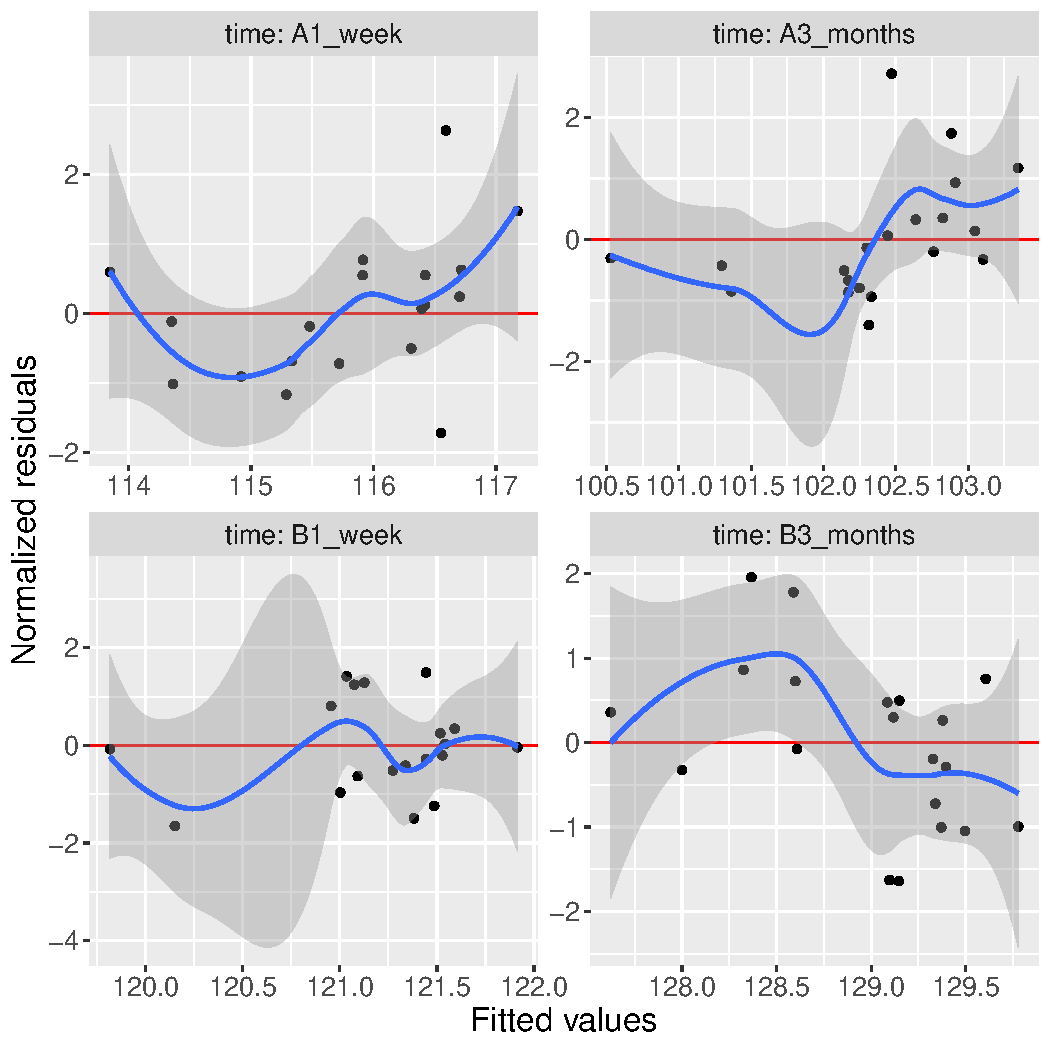
\includegraphics[width=0.4\textwidth]{./figures/diag-scatterplot.pdf}
\end{center}

\begin{itemize}
\item misspecification of the variance structure
\end{itemize}
\lstset{language=r,label= ,caption= ,captionpos=b,numbers=none}
\begin{lstlisting}
plot(eUN.lmm, type = "scatterplot2")
\end{lstlisting}

\begin{center}
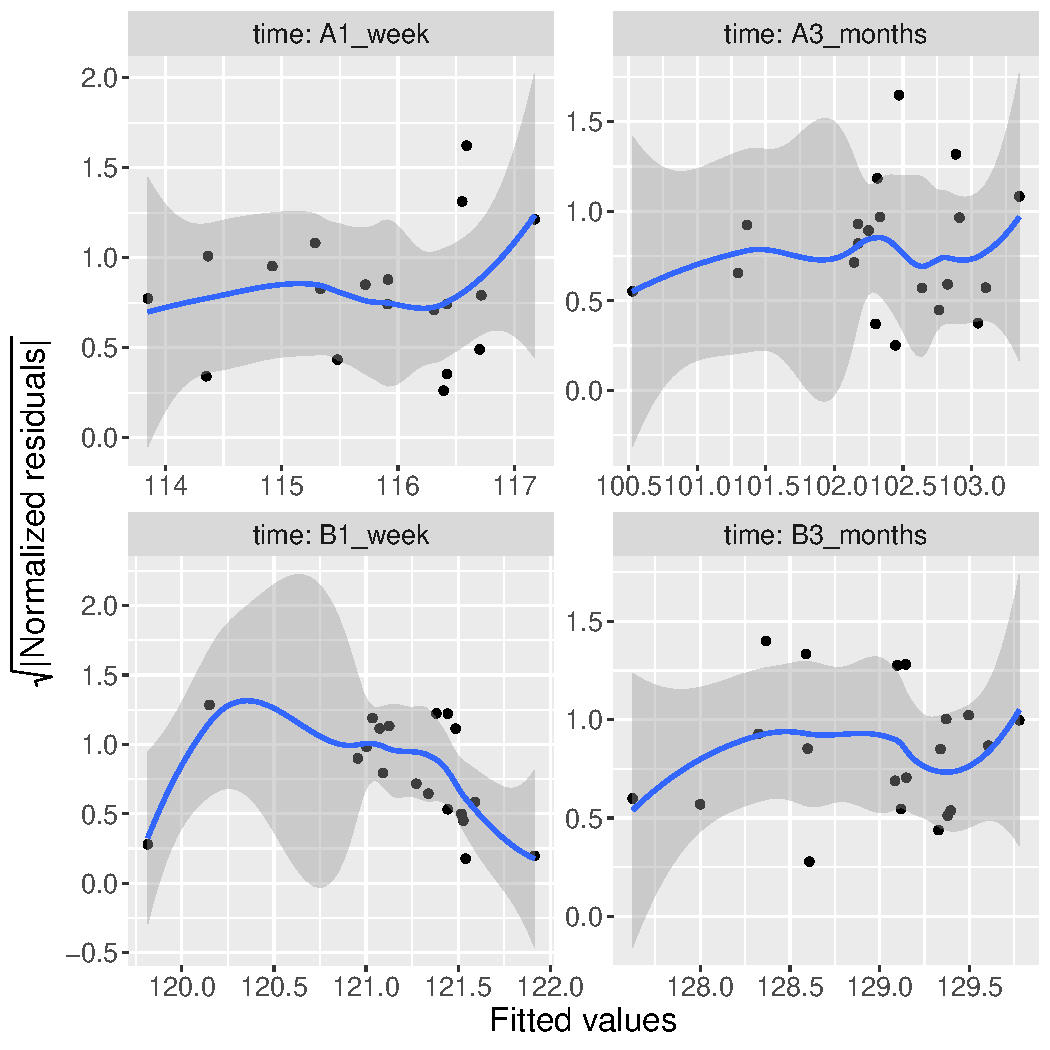
\includegraphics[width=0.4\textwidth]{./figures/diag-scatterplot2.pdf}
\end{center}

\clearpage

\begin{itemize}
\item misspecification of the correlation structure
\end{itemize}

\lstset{language=r,label= ,caption= ,captionpos=b,numbers=none}
\begin{lstlisting}
plot(eUN.lmm, type = "correlation", type.residual = "response")
plot(eUN.lmm, type = "correlation", type.residual = "normalized")
\end{lstlisting}

\begin{center}
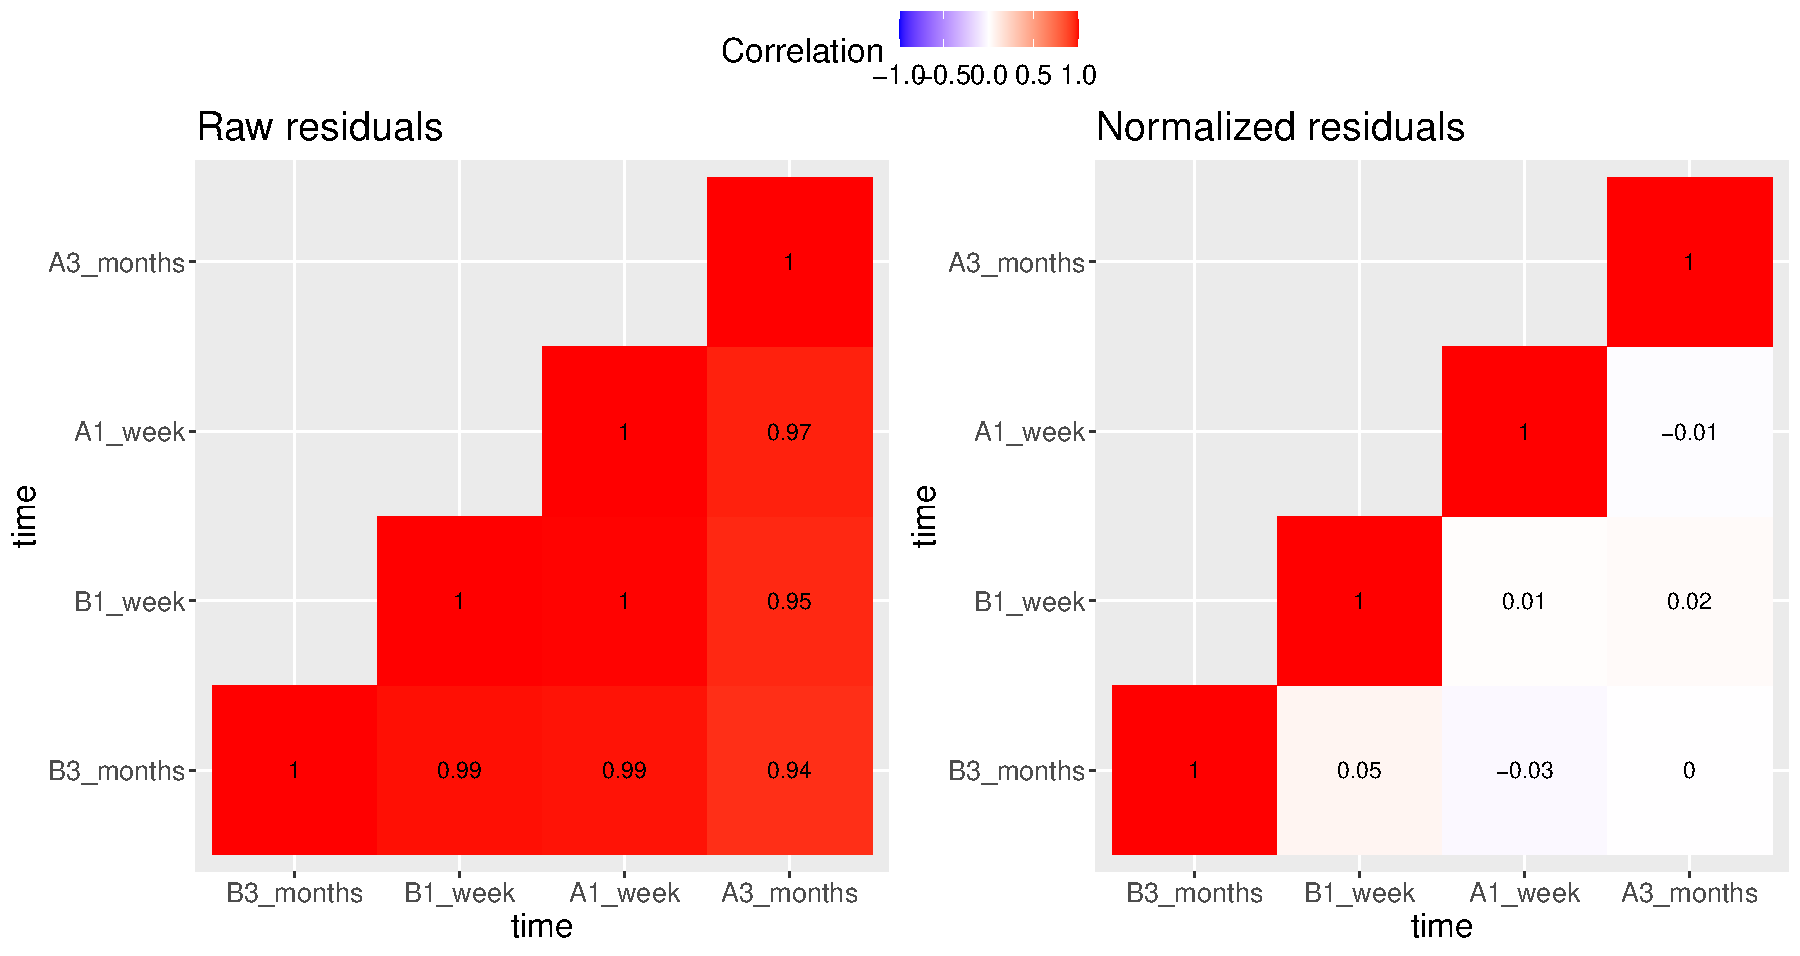
\includegraphics[width=0.6\textwidth]{./figures/diag-correlation.pdf}
\end{center}

\begin{itemize}
\item residual distribution vs. normal distribution \footnote{see \cite{oldford2016self} for guidance
about how to read quantile-quantile plots.}:
\end{itemize}
\lstset{language=r,label= ,caption= ,captionpos=b,numbers=none}
\begin{lstlisting}
plot(eUN.lmm, type = "qqplot", engine.qqplot = "qqtest")
## Note: the qqtest package to be installed to use the argument engine.plot = "qqtest" 
\end{lstlisting}

\begin{center}
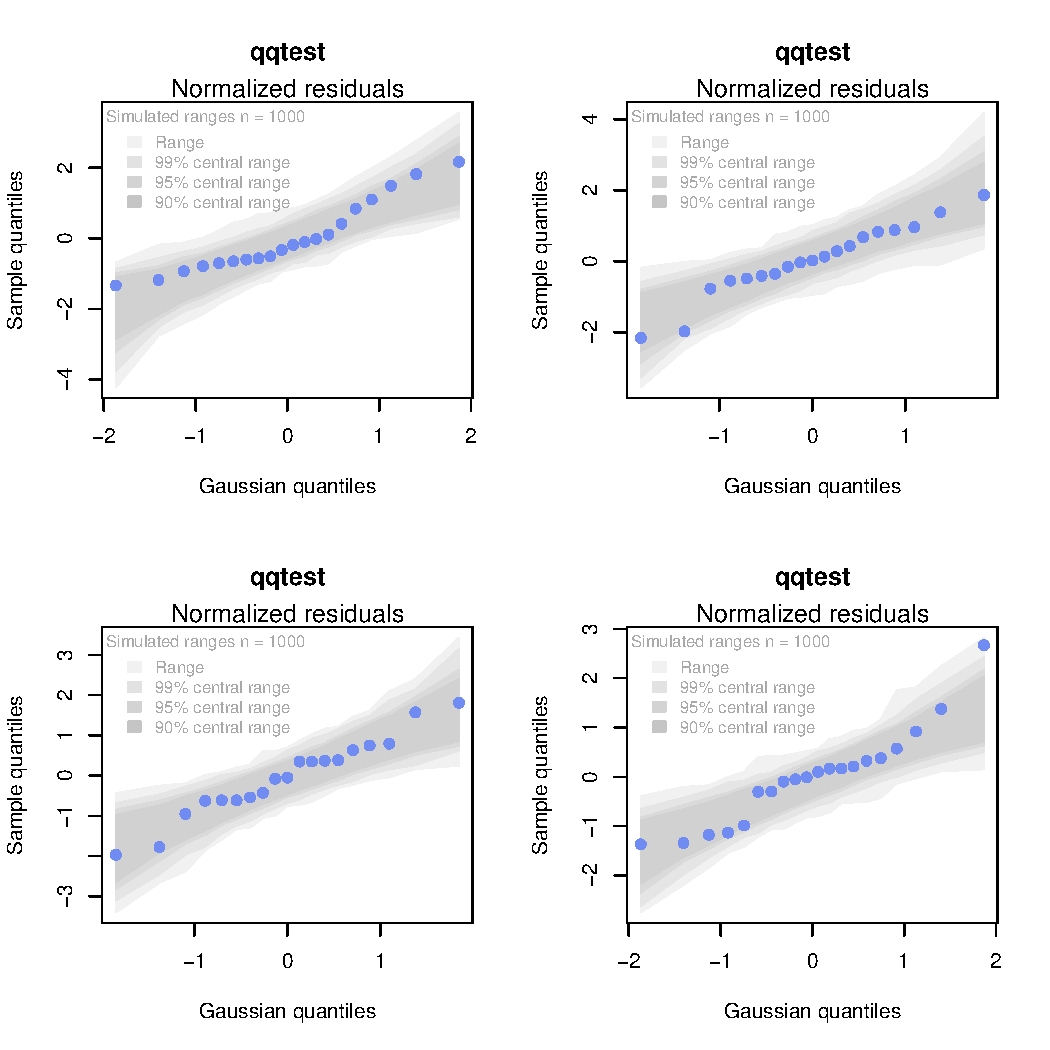
\includegraphics[width=0.5\textwidth]{./figures/diag-qqplot.pdf}
\end{center}

\clearpage

The method \texttt{residuals} returns the residulas in the wide format:
\lstset{language=r,label= ,caption= ,captionpos=b,numbers=none}
\begin{lstlisting}
eUN.diagW <- residuals(eUN.lmm, type = "normalized", format = "wide")
colnames(eUN.diagW) <- gsub("normalized.","",colnames(eUN.diagW))
head(eUN.diagW)
\end{lstlisting}

\begin{verbatim}
  cluster r.B3_months  r.B1_week   r.A1_week r.A3_months
1       1  -0.2897364 -0.2027622 -1.16864032   0.3258573
2       2   0.8603118 -1.6492167  0.62578804   1.7370660
3       3   0.7273066 -0.4155168 -0.68266746  -0.8510316
4       4  -1.6403081 -0.5128371  0.06806211   1.1725813
5       5   0.4755409         NA -0.18736417  -0.8634200
6       6   1.7801675  1.2847698  2.63004809   0.3505542
\end{verbatim}


or in the long format:
\lstset{language=r,label= ,caption= ,captionpos=b,numbers=none}
\begin{lstlisting}
eUN.diagL <- residuals(eUN.lmm, type = "normalized", format = "long")
head(eUN.diagL)
\end{lstlisting}

\begin{verbatim}
[1] -0.2897364  0.8603118  0.7273066 -1.6403081  0.4755409  1.7801675
\end{verbatim}


Various type of residuals can be extract but the normalized one are
recommanded when doing model checking.

\subsection{Model fit}
\label{sec:org9ba55da}

The fitted values can be displayed via the \texttt{plot} method or using the \texttt{emmeans} package:

\lstset{language=r,label= ,caption= ,captionpos=b,numbers=none}
\begin{lstlisting}
library(ggplot2) ## left panel
autoplot(eUN.lmm, color = "id", size.text = 20)
\end{lstlisting}

\lstset{language=r,label= ,caption= ,captionpos=b,numbers=none}
\begin{lstlisting}
library(emmeans) ## right panel
emmip(eUN.lmm, ~time) + theme(text = element_text(size=20))
\end{lstlisting}

\begin{minipage}{0.45\linewidth}
\begin{center}
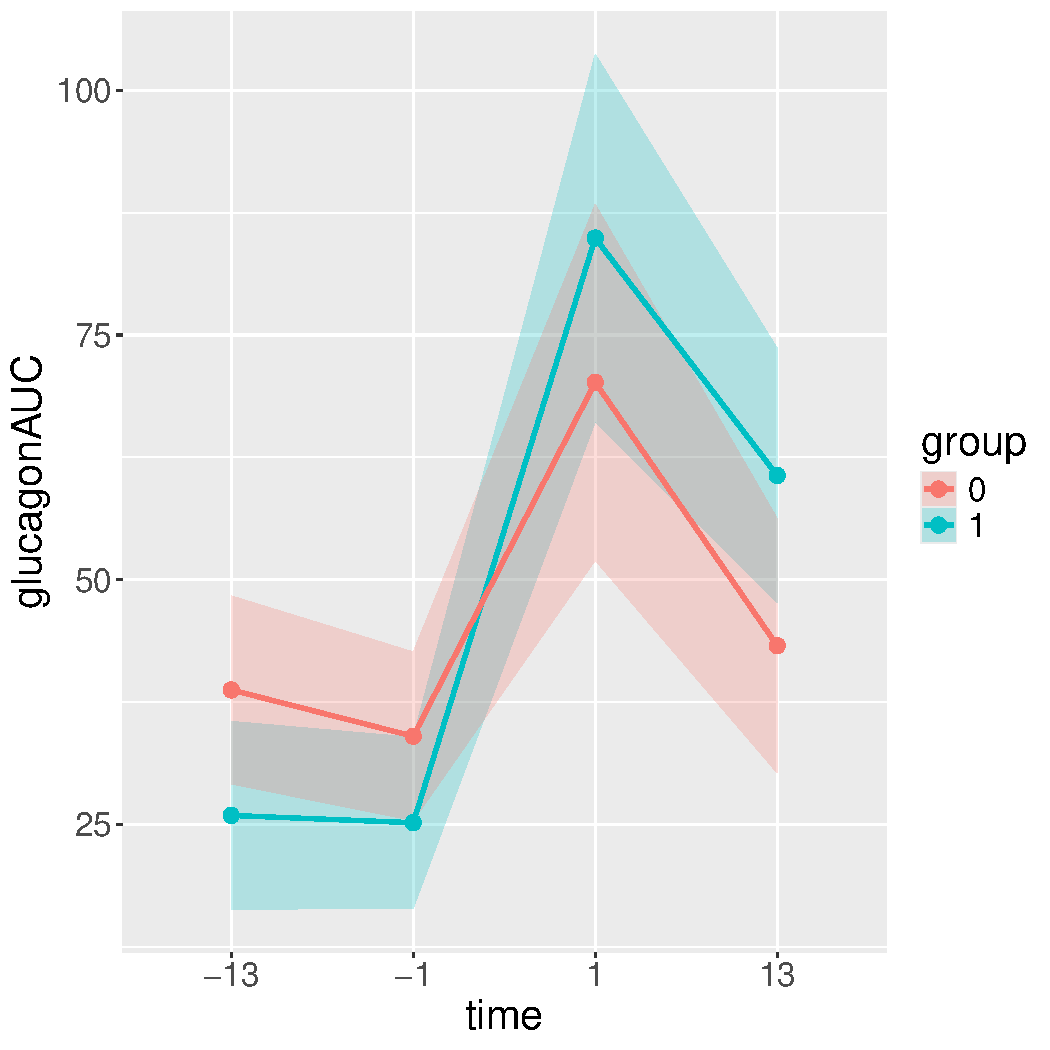
\includegraphics[width=\textwidth]{./figures/fit-autoplot.pdf}
\end{center}
\end{minipage}
\begin{minipage}{0.45\linewidth}
\begin{center}
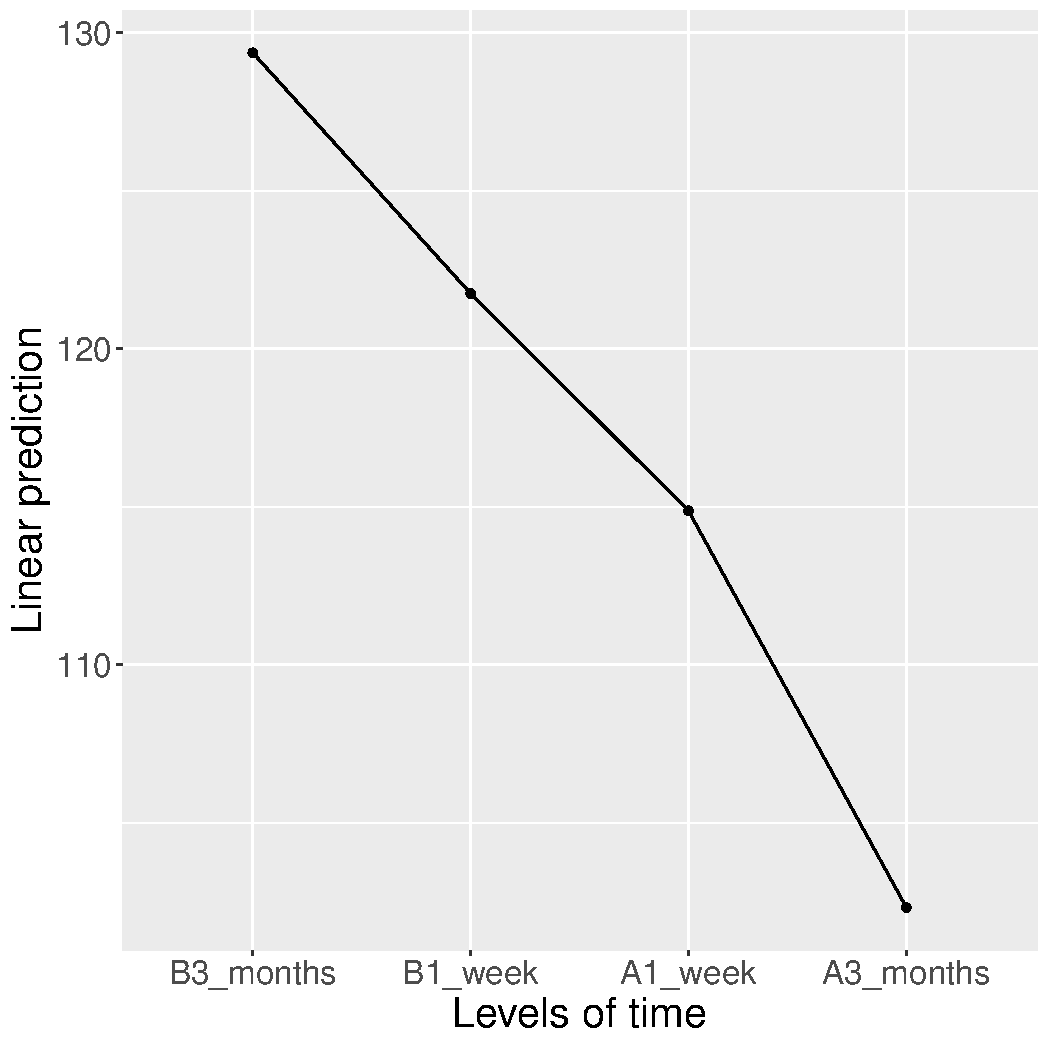
\includegraphics[width=\textwidth]{./figures/fit-emmip.pdf}
\end{center}
\end{minipage}

In the first case each possible curve is displayed while in the latter
the average curve (over glucagon values). With the \texttt{autoplot} method,
it is possible to display a curve specific to a glucagon value via the
argument \texttt{at}:
\lstset{language=r,label= ,caption= ,captionpos=b,numbers=none}
\begin{lstlisting}
autoplot(eUN.lmm, at = data.frame(glucagon = 10), color = "glucagon")
\end{lstlisting}

\subsection{Statistical inference}
\label{sec:orge7f6d0b}

The \texttt{anova} method can be use to test one or several linear
combinations of the model coefficients using Wald tests. By default,
it will simultaneously test all parameters associated to a variable:
\lstset{language=r,label= ,caption= ,captionpos=b,numbers=none}
\begin{lstlisting}
anova(eUN.lmm)
\end{lstlisting}

\begin{verbatim}
                     ** mean coefficients ** 
 - F-test
         statistic df.num df.denom      p.value
time      86.74280      3 19.00520 2.842460e-11
glucagon  13.51775      1 13.70749 2.571626e-03
\end{verbatim}


Note that here the p-values are not adjust for multiple comparisons
over variables. It is possible to specify a null hypothesis to be
test: e.g. is there a change in average weight just after taking the
treatment:
\lstset{language=r,label= ,caption= ,captionpos=b,numbers=none}
\begin{lstlisting}
anova(eUN.lmm, effects = c("timeA1_week-timeB1_week=0"), ci = TRUE)
\end{lstlisting}

\begin{verbatim}
                     ** User-specified hypotheses ** 
 - F-test
 statistic df.num df.denom      p.value
  43.14135      1 17.87455 3.723358e-06

 - P-values and confidence interval 
                           estimate     lower     upper      p.value
timeA1_week - timeB1_week -3.905721 -5.155643 -2.655799 3.723358e-06
\end{verbatim}


One can also simulateneously tests several null hypotheses:
\lstset{language=r,label= ,caption= ,captionpos=b,numbers=none}
\begin{lstlisting}
anova(eUN.lmm, effects = c("timeA1_week-timeB1_week=0",
			   "timeA3_months-timeB1_week=0"), ci = TRUE)
\end{lstlisting}

\begin{verbatim}
                     ** User-specified hypotheses ** 
 - F-test
 statistic df.num df.denom     p.value
  98.65054      2 18.61992 1.23382e-10

 - P-values and confidence interval (adjusted for multiplicity) 
                              estimate      lower      upper      p.value
timeA1_week - timeB1_week    -3.905721  -5.306911  -2.504531 4.080425e-06
timeA3_months - timeB1_week -18.240158 -21.357228 -15.123087 2.195166e-11
\end{verbatim}


When testing transformed variance or correlation parameters,
parentheses (as in \texttt{log(k).B1\_week}) cause problem for recognizing
parameters:
\lstset{language=r,label= ,caption= ,captionpos=b,numbers=none}
\begin{lstlisting}
try(
  anova(eUN.lmm,
	effects = c("log(k).B1_week=0","log(k).A1_week=0","log(k).A3_months=0"))
)
\end{lstlisting}

\begin{verbatim}
Error in .anova_Wald(object, effects = effects, rhs = rhs, df = df, ci = ci,  : 
  Possible mispecification of the argument 'effects' as running mulcomp::glht lead to the following error: 
Error in parse(text = ex[i]) : <text>:1:7: uventet symbol
1: log(k).B1_week
          ^
\end{verbatim}


It is then advised to build a contrast matrix, e.g.:
\lstset{language=r,label= ,caption= ,captionpos=b,numbers=none}
\begin{lstlisting}
name.coef <- rownames(confint(eUN.lmm, effects = "all", backtransform = FALSE))
name.varcoef <- grep("log(k)",name.coef, value = TRUE, fixed = TRUE)
C <- matrix(0, nrow = 3, ncol = length(name.coef), dimnames = list(name.varcoef, name.coef))
diag(C[name.varcoef,name.varcoef]) <- 1
C
\end{lstlisting}

\begin{verbatim}
                 (Intercept) timeB1_week timeA1_week timeA3_months glucagon log(sigma)
log(k).B1_week             0           0           0             0        0          0
log(k).A1_week             0           0           0             0        0          0
log(k).A3_months           0           0           0             0        0          0
                 log(k).B1_week log(k).A1_week log(k).A3_months atanh(rho(B3_months,B1_week))
log(k).B1_week                1              0                0                             0
log(k).A1_week                0              1                0                             0
log(k).A3_months              0              0                1                             0
                 atanh(rho(B3_months,A1_week)) atanh(rho(B3_months,A3_months))
log(k).B1_week                               0                               0
log(k).A1_week                               0                               0
log(k).A3_months                             0                               0
                 atanh(rho(B1_week,A1_week)) atanh(rho(B1_week,A3_months))
log(k).B1_week                             0                             0
log(k).A1_week                             0                             0
log(k).A3_months                           0                             0
                 atanh(rho(A1_week,A3_months))
log(k).B1_week                               0
log(k).A1_week                               0
log(k).A3_months                             0
\end{verbatim}

And then call the \texttt{anova} method specifying the null hypothesis via the
contrast matrix:
\lstset{language=r,label= ,caption= ,captionpos=b,numbers=none}
\begin{lstlisting}
anova(eUN.lmm, effects = C)
\end{lstlisting}

\begin{verbatim}
                    ** User-specified hypotheses ** 
- F-test
statistic df.num df.denom     p.value
 6.203161      3 17.99456 0.004417117
\end{verbatim}


\clearpage

\subsection{Baseline adjustment}
\label{sec:org3a0a9d5}

The \texttt{lmm} contains an "experimental" feature to drop non-identifiable
effects from the model. For instance, let us define two (artifical) groups of
patients:
\lstset{language=r,label= ,caption= ,captionpos=b,numbers=none}
\begin{lstlisting}
gastricbypassL$group <- c("1","2")[as.numeric(gastricbypassL$id) %in% 15:20 + 1]
\end{lstlisting}
We would like to model group differences only after baseline
(i.e. only at 1 week and 3 months after). For this we will define a
treatment variable being the group variable except before baseline where
it is \texttt{"none"}:
\lstset{language=r,label= ,caption= ,captionpos=b,numbers=none}
\begin{lstlisting}
gastricbypassL$treat <- baselineAdjustment(gastricbypassL, variable = "group",
					   repetition = ~time|id, constrain = c("B3_months","B1_week"),
					   new.level = "none")
table(treat = gastricbypassL$treat, time = gastricbypassL$time, group = gastricbypassL$group)
\end{lstlisting}

\begin{verbatim}
, , group = 1

      time
treat  B3_months B1_week A1_week A3_months
  none        14      14       0         0
  1            0       0      14        14
  2            0       0       0         0

, , group = 2

      time
treat  B3_months B1_week A1_week A3_months
  none         6       6       0         0
  1            0       0       0         0
  2            0       0       6         6
\end{verbatim}

Here we will be able to estimate a total of 6 means and therefore can
at most identify 6 effects. However the design matrix for the
interaction model:
\lstset{language=r,label= ,caption= ,captionpos=b,numbers=none}
\begin{lstlisting}
colnames(model.matrix(weight ~ treat*time, data = gastricbypassL))
\end{lstlisting}

\begin{verbatim}
[1] "(Intercept)"          "treat1"               "treat2"               "timeB1_week"         
[5] "timeA1_week"          "timeA3_months"        "treat1:timeB1_week"   "treat2:timeB1_week"  
[9] "treat1:timeA1_week"   "treat2:timeA1_week"   "treat1:timeA3_months" "treat2:timeA3_months"
\end{verbatim}


contains 12 parameters (i.e. 6 too many). The \texttt{lmm} function will
internally remove the one that cannot be identified and fit a
simplified model:
\lstset{language=r,label= ,caption= ,captionpos=b,numbers=none}
\begin{lstlisting}
eC.lmm <- lmm(weight ~ treat*time, data = gastricbypassL,
	      repetition = ~time|id, structure = "UN")
\end{lstlisting}

\begin{verbatim}
Constant values in the design matrix in interactions "treat:time"
 Coefficients "treat1" "treat2" "timeA1_week" "timeA3_months" "treat1:timeB1_week" "treat2:timeB1_week" have been removed.
\end{verbatim}


with the following coefficients:
\lstset{language=r,label= ,caption= ,captionpos=b,numbers=none}
\begin{lstlisting}
coef(eC.lmm, effects = "mean")
\end{lstlisting}

\begin{verbatim}
         (Intercept)          timeB1_week   treat1:timeA1_week   treat2:timeA1_week 
           128.97000             -7.73000            -12.83949            -14.27452 
treat1:timeA3_months treat2:timeA3_months 
           -27.07620            -25.50553
\end{verbatim}


One can vizualize the baseline adjustment via the \texttt{autoplot} function:
\lstset{language=r,label= ,caption= ,captionpos=b,numbers=none}
\begin{lstlisting}
autoplot(eC.lmm, color = "group", ci = FALSE, size.text = 20)
\end{lstlisting}

\begin{center}
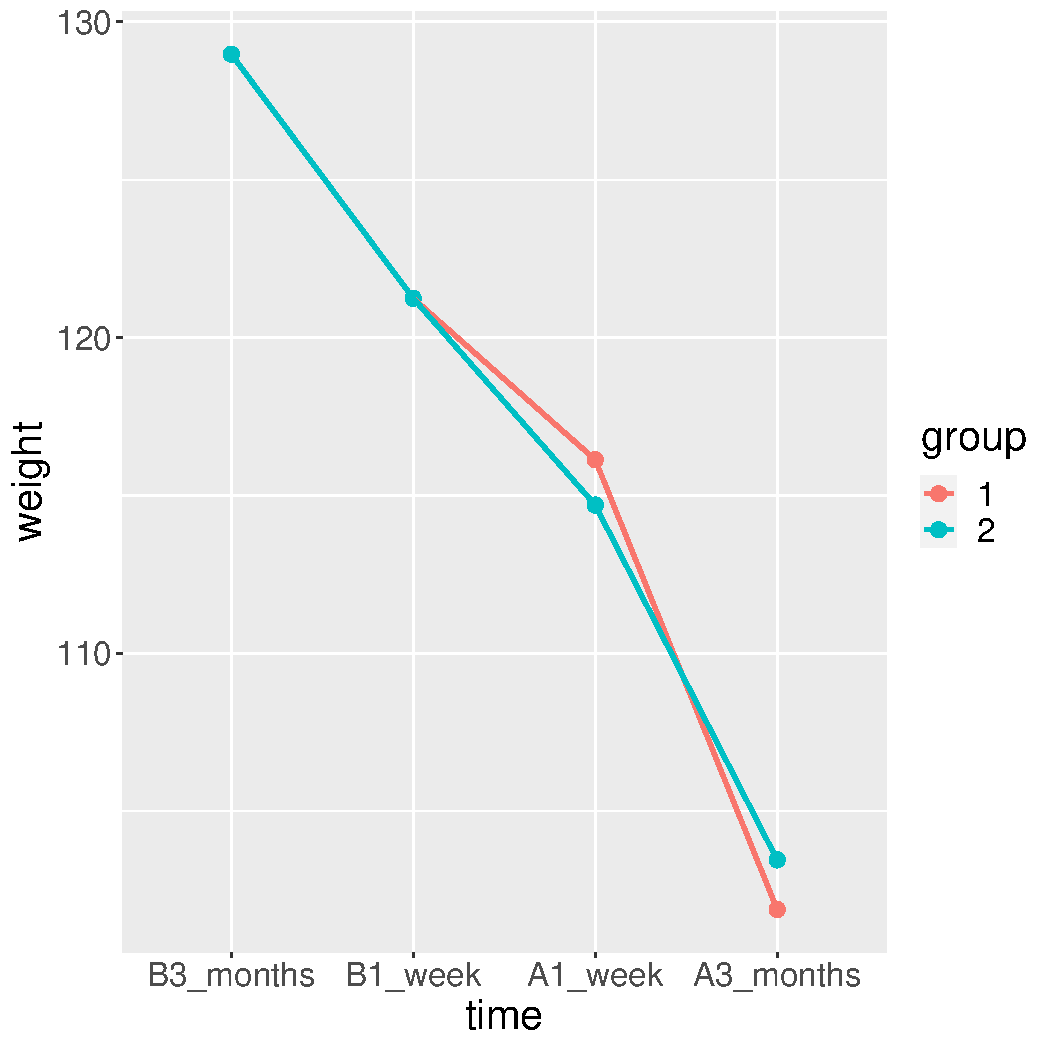
\includegraphics[width=0.4\textwidth]{./figures/gg-baseAdj.pdf}
\end{center}

To more easily compare the two groups, one could set the baseline
treatment to the treatment in the control arm by omitting the argument
\texttt{new.level}:
\lstset{language=r,label= ,caption= ,captionpos=b,numbers=none}
\begin{lstlisting}
gastricbypassL$treat2 <- baselineAdjustment(gastricbypassL, variable = "group",
					    repetition = ~time|id, constrain = c("B3_months","B1_week"))
table(treat = gastricbypassL$treat2, time = gastricbypassL$time, group = gastricbypassL$group)
\end{lstlisting}

\begin{verbatim}
windows 
      2
, , group = 1

     time
treat B3_months B1_week A1_week A3_months
    1        14      14      14        14
    2         0       0       0         0

, , group = 2

     time
treat B3_months B1_week A1_week A3_months
    1         6       6       0         0
    2         0       0       6         6
\end{verbatim}

Fitting the model
\lstset{language=r,label= ,caption= ,captionpos=b,numbers=none}
\begin{lstlisting}
eC2.lmm <- suppressWarnings(lmm(weight ~ treat2*time, data = gastricbypassL,
				repetition = ~time|id, structure = "UN"))
\end{lstlisting}

\begin{verbatim}
Constant values in the design matrix in interactions "treat2:time"
 Coefficients "treat22" "treat22:timeB1_week" have been removed.
\end{verbatim}


will directly output group differences (last two coefficients):
\lstset{language=r,label= ,caption= ,captionpos=b,numbers=none}
\begin{lstlisting}
model.tables(eC2.lmm)
\end{lstlisting}
\begin{verbatim}
                      estimate    se   df  lower  upper  p.value
(Intercept)             128.97 4.532 19.0 119.48 138.46 0.00e+00
timeB1_week              -7.73 0.697 19.0  -9.19  -6.27 1.00e-09
timeA1_week             -12.84 0.865 20.5 -14.64 -11.04 2.02e-12
timeA3_months           -27.08 1.724 21.4 -30.66 -23.50 3.20e-13
treat22:timeA1_week      -1.44 0.621 16.3  -2.75  -0.12 3.43e-02
treat22:timeA3_months     1.57 2.463 16.3  -3.64   6.78 5.32e-01
\end{verbatim}


It is also possible to get the estimated mean at each timepoint, using
an equivalent mean structure:
\lstset{language=r,label= ,caption= ,captionpos=b,numbers=none}
\begin{lstlisting}
eC3.lmm <- suppressWarnings(lmm(weight ~ 0+treat2:time, data = gastricbypassL,
				repetition = ~time|id, structure = "UN"))
model.tables(eC3.lmm) ## equivalent to dummy.coef(eC2.lmm)
\end{lstlisting}

\begin{verbatim}
Constant values in the design matrix in interactions "treat2:time"
 Coefficients "treat22:timeB3_months" "treat22:timeB1_week" have been removed.
                      estimate   se   df lower upper p.value
treat21:timeB3_months      129 4.53 19.0 119.5   138       0
treat21:timeB1_week        121 4.23 19.0 112.4   130       0
treat21:timeA1_week        116 4.11 19.1 107.5   125       0
treat22:timeA1_week        115 4.13 19.4 106.1   123       0
treat21:timeA3_months      102 3.87 20.2  93.8   110       0
treat22:timeA3_months      103 4.17 25.2  94.9   112       0
\end{verbatim}


or the baseline mean and the change since baseline:
\lstset{language=r,label= ,caption= ,captionpos=b,numbers=none}
\begin{lstlisting}
eC4.lmm <- suppressWarnings(lmm(weight ~ treat2:time, data = gastricbypassL,
				repetition = ~time|id, structure = "UN"))
model.tables(eC4.lmm)
\end{lstlisting}

\begin{verbatim}
Constant values in the design matrix in interactions "treat2:time"
 Coefficients "treat22:timeB3_months" "treat22:timeB1_week" have been removed.
                      estimate    se   df  lower  upper  p.value
(Intercept)             128.97 4.532 19.0 119.48 138.46 0.00e+00
treat21:timeB1_week      -7.73 0.697 19.0  -9.19  -6.27 1.00e-09
treat21:timeA1_week     -12.84 0.865 20.5 -14.64 -11.04 2.02e-12
treat22:timeA1_week     -14.27 0.950 26.3 -16.23 -12.32 2.02e-14
treat21:timeA3_months   -27.08 1.724 21.4 -30.66 -23.50 3.20e-13
treat22:timeA3_months   -25.51 2.323 22.6 -30.32 -20.69 1.60e-10
\end{verbatim}

\subsection{Marginal means}
\label{sec:org35a66fc}

The \texttt{emmeans} package can be used to output marginal means. Consider
the following model:
\lstset{language=r,label= ,caption= ,captionpos=b,numbers=none}
\begin{lstlisting}
e.group <- lmm(weight ~ time*group, data = gastricbypassL,
	       repetition = ~time|id, structure = "UN")
\end{lstlisting}

We can for instance compute the average value over time \emph{assuming balanced groups}:
\lstset{language=r,label= ,caption= ,captionpos=b,numbers=none}
\begin{lstlisting}
emmeans(e.group, specs=~time)
\end{lstlisting}

\begin{verbatim}
NOTE: Results may be misleading due to involvement in interactions
 time      emmean   SE   df lower.CL upper.CL
 B3_months    130 5.05 18.0    119.3      141
 B1_week      122 4.69 18.0    112.5      132
 A1_week      117 4.55 18.0    107.0      126
 A3_months    104 4.20 18.1     94.9      113

Results are averaged over the levels of: group 
Confidence level used: 0.95
\end{verbatim}


This differs from the average value over time over the whole sample:
\lstset{language=r,label= ,caption= ,captionpos=b,numbers=none}
\begin{lstlisting}
df.pred <- cbind(gastricbypassL, predict(e.group, newdata = gastricbypassL))
summarize(formula = estimate~time, data = df.pred)
\end{lstlisting}

\begin{verbatim}
   outcome      time observed missing    mean       sd      min   median    max
1 estimate B3_months       20       0 128.970 2.270212 127.5214 127.5214 132.35
2 estimate   B1_week       20       0 121.240 2.726942 119.5000 119.5000 125.30
3 estimate   A1_week       20       0 115.700 2.014981 114.4143 114.4143 118.70
4 estimate A3_months       20       0 102.365 3.146729 100.3571 100.3571 107.05
\end{verbatim}


as the groups are not balanced:
\lstset{language=r,label= ,caption= ,captionpos=b,numbers=none}
\begin{lstlisting}
table(group = gastricbypassL$group, time = gastricbypassL$time)
\end{lstlisting}

\begin{verbatim}
     time
group B3_months B1_week A1_week A3_months
    1        14      14      14        14
    2         6       6       6         6
\end{verbatim}


The "emmeans" approach gives equal "weight" to the expected value of
both group 2:
\lstset{language=r,label= ,caption= ,captionpos=b,numbers=none}
\begin{lstlisting}
mu.group1 <-  as.double(coef(e.group)["(Intercept)"])
mu.group2 <-  as.double(coef(e.group)["(Intercept)"] + coef(e.group)["group2"])
p.group1 <- 14/20          ; p.group2 <- 6/20
c(emmeans = (mu.group1+mu.group2)/2, predict = mu.group1 * p.group1 + mu.group2 * p.group2)
\end{lstlisting}

\begin{verbatim}
 emmeans  predict 
129.9357 128.9700
\end{verbatim}


Which one is relevant depends on the application. The \texttt{emmeans}
function can also be used to display expected value in each group over
time:
\lstset{language=r,label= ,caption= ,captionpos=b,numbers=none}
\begin{lstlisting}
emmeans.group <- emmeans(e.group, specs = ~group|time)
emmeans.group
\end{lstlisting}

\begin{verbatim}
time = B3_months:
 group emmean   SE   df lower.CL upper.CL
 1        128 5.53 18.0    115.9      139
 2        132 8.45 18.0    114.6      150

time = B1_week:
 group emmean   SE   df lower.CL upper.CL
 1        120 5.14 18.0    108.7      130
 2        125 7.85 18.0    108.8      142

time = A1_week:
 group emmean   SE   df lower.CL upper.CL
 1        114 4.99 18.0    103.9      125
 2        119 7.62 18.0    102.7      135

time = A3_months:
 group emmean   SE   df lower.CL upper.CL
 1        100 4.60 18.1     90.7      110
 2        107 7.03 18.1     92.3      122

Confidence level used: 0.95
\end{verbatim}

Using the \texttt{pair} function displays the differences:
\lstset{language=r,label= ,caption= ,captionpos=b,numbers=none}
\begin{lstlisting}
epairs.group <- pairs(emmeans.group, reverse = TRUE)
epairs.group
\end{lstlisting}

\begin{verbatim}
time = B3_months:
 contrast estimate    SE   df t.ratio p.value
 2 - 1        4.83 10.10 18.0   0.478  0.6383

time = B1_week:
 contrast estimate    SE   df t.ratio p.value
 2 - 1        5.80  9.38 18.0   0.618  0.5441

time = A1_week:
 contrast estimate    SE   df t.ratio p.value
 2 - 1        4.29  9.11 18.0   0.471  0.6435

time = A3_months:
 contrast estimate    SE   df t.ratio p.value
 2 - 1        6.69  8.40 18.1   0.797  0.4361
\end{verbatim}

One can adjust for multiple comparison via the \texttt{adjust} argument and
display confidence intervals setting the argument \texttt{infer} to \texttt{TRUE}:
\lstset{language=r,label= ,caption= ,captionpos=b,numbers=none}
\begin{lstlisting}
summary(epairs.group, by = NULL, adjust = "mvt", infer = TRUE)
\end{lstlisting}

\begin{verbatim}
 contrast time      estimate    SE   df lower.CL upper.CL t.ratio p.value
 2 - 1    B3_months     4.83 10.10 18.0    -18.0     27.6   0.478  0.7493
 2 - 1    B1_week       5.80  9.38 18.0    -15.4     27.0   0.618  0.6479
 2 - 1    A1_week       4.29  9.11 18.0    -16.3     24.8   0.471  0.7550
 2 - 1    A3_months     6.69  8.40 18.1    -12.3     25.7   0.797  0.5284

Confidence level used: 0.95 
Conf-level adjustment: mvt method for 4 estimates 
P value adjustment: mvt method for 4 tests
\end{verbatim}


This should also work when doing baseline adjustment (because of
baseline adjustment no difference is expected at the first two
timepoints):
\lstset{language=r,label= ,caption= ,captionpos=b,numbers=none}
\begin{lstlisting}
summary(pairs(emmeans(eC2.lmm , specs = ~treat2|time), reverse = TRUE), by = NULL)
\end{lstlisting}

\begin{verbatim}
Note: adjust = "tukey" was changed to "sidak"
because "tukey" is only appropriate for one set of pairwise comparisons
 contrast time      estimate    SE   df t.ratio p.value
 2 - 1    B3_months     0.00 0.000  NaN     NaN     NaN
 2 - 1    B1_week       0.00 0.000  NaN     NaN     NaN
 2 - 1    A1_week      -1.44 0.621 16.2  -2.311  0.1303
 2 - 1    A3_months     1.57 2.463 16.3   0.638  0.9522

P value adjustment: sidak method for 4 tests
\end{verbatim}

\subsection{Predictions}
\label{sec:orge02cee2}

Two types of predictions can be performed with the \texttt{predict} method:
\begin{itemize}
\item \textbf{static predictions} that are only conditional on the covariates:
\end{itemize}
\lstset{language=r,label= ,caption= ,captionpos=b,numbers=none}
\begin{lstlisting}
news <- gastricbypassL[gastricbypassL$id==1,]
news$glucagon <- 0
predict(eUN.lmm, newdata = news)
\end{lstlisting}

\begin{verbatim}
  estimate       se       df     lower    upper
1 128.5386 4.536445 18.97584 119.04289 138.0343
2 120.6564 4.261691 19.04078 111.73783 129.5749
3 116.7506 3.956964 19.04925 108.47007 125.0312
4 102.4162 3.747908 19.05531  94.57328 110.2591
\end{verbatim}


\clearpage

which can be computing by creating a design matrix:
\lstset{language=r,label= ,caption= ,captionpos=b,numbers=none}
\begin{lstlisting}
X.12 <- model.matrix(formula(eUN.lmm), news)
X.12
\end{lstlisting}

\begin{verbatim}
   (Intercept) timeB1_week timeA1_week timeA3_months glucagon
1            1           0           0             0        0
21           1           1           0             0        0
41           1           0           1             0        0
61           1           0           0             1        0
attr(,"assign")
[1] 0 1 1 1 2
attr(,"contrasts")
attr(,"contrasts")$time
[1] "contr.treatment"
\end{verbatim}

and then multiplying it with the regression coefficients:
\lstset{language=r,label= ,caption= ,captionpos=b,numbers=none}
\begin{lstlisting}
X.12 %*% coef(eUN.lmm)
\end{lstlisting}

\begin{verbatim}
       [,1]
1  128.5386
21 120.6564
41 116.7506
61 102.4162
\end{verbatim}


\begin{itemize}
\item \textbf{dynamic predictions} that are conditional on the covariates and the
outcome measured at other timepoints. Consider two subjects for who
we would like to predict the weight 1 week before the intervention
based on the weight 3 months before the intervention:
\end{itemize}

\lstset{language=r,label= ,caption= ,captionpos=b,numbers=none,otherkeywords={}, deletekeywords={}}
\begin{lstlisting}
newd <- rbind(
  data.frame(id = 1, time = "B3_months", weight = coef(eUN.lmm)["(Intercept)"], glucagon = 0),
  data.frame(id = 1, time = "B1_week", weight = NA, glucagon = 0),
  data.frame(id = 2, time = "B3_months", weight = 100, glucagon = 0),
  data.frame(id = 2, time = "B1_week", weight = NA, glucagon = 0)
)
predict(eUN.lmm, newdata = newd, type = "dynamic", keep.newdata = TRUE)
\end{lstlisting}

\begin{verbatim}
  id      time   weight glucagon  estimate        se  df     lower    upper
1  1 B3_months 128.5386        0        NA        NA  NA        NA       NA
2  1   B1_week       NA        0 120.65636 0.6361008 Inf 119.40963 121.9031
3  2 B3_months 100.0000        0        NA        NA  NA        NA       NA
4  2   B1_week       NA        0  94.15336 6.2597469 Inf  81.88448 106.4222
\end{verbatim}


The first subjects has the average weight while the second has a much
  lower weight. The predicted weight for the first subject is then the
  average weight one week before while it is lower for the second
  subject due to the positive correlation over time. The predicted
  value is computed using the formula of the conditional mean for a
  Gaussian vector:
\lstset{language=r,label= ,caption= ,captionpos=b,numbers=none}
\begin{lstlisting}
mu1 <- coef(eUN.lmm)[1]
mu2 <- sum(coef(eUN.lmm)[1:2])
Omega_11 <- getVarCov(eUN.lmm)["B3_months","B3_months"]
Omega_21 <- getVarCov(eUN.lmm)["B1_week","B3_months"]
as.double(mu2 + Omega_21 * (100 - mu1) / Omega_11)
\end{lstlisting}

\begin{verbatim}
[1] 94.15336
\end{verbatim}



\clearpage

\section{Data generation}
\label{sec:org4e7986a}
Simulate some data in the wide format:
\lstset{language=r,label= ,caption= ,captionpos=b,numbers=none}
\begin{lstlisting}
set.seed(10) ## ensure reproductibility
n.obs <- 100
n.times <- 4
mu <- rep(0,4)
gamma <- matrix(0, nrow = n.times, ncol = 10) ## add interaction
gamma[,6] <- c(0,1,1.5,1.5)
dW <- sampleRem(n.obs, n.times = n.times, mu = mu, gamma = gamma, format = "wide")
head(round(dW,3))
\end{lstlisting}

\begin{verbatim}
  id X1 X2 X3 X4 X5     X6     X7     X8    X9    X10     Y1     Y2     Y3     Y4
1  1  1  0  1  1  0 -0.367  1.534 -1.894 1.729  0.959  1.791  2.429  3.958  2.991
2  2  1  0  1  2  0 -0.410  2.065  1.766 0.761 -0.563  2.500  4.272  3.002  2.019
3  3  0  0  2  1  0 -1.720 -0.178  2.357 1.966  1.215 -3.208 -5.908 -4.277 -5.154
4  4  0  0  0  1  0  0.923 -2.089  0.233 1.307 -0.906 -2.062  0.397  1.757 -1.380
5  5  0  0  2  1  0  0.987  5.880  0.385 0.028  0.820  7.963  7.870  7.388  8.609
6  6  0  0  1  1  2 -1.075  0.479  2.202 0.900 -0.739  0.109 -1.602 -1.496 -1.841
\end{verbatim}


Simulate some data in the long format:
\lstset{language=r,label= ,caption= ,captionpos=b,numbers=none}
\begin{lstlisting}
set.seed(10) ## ensure reproductibility
dL <- sampleRem(n.obs, n.times = n.times, mu = mu, gamma = gamma, format = "long")
head(dL)
\end{lstlisting}

\begin{verbatim}
  id visit        Y X1 X2 X3 X4 X5         X6       X7        X8        X9        X10
1  1     1 1.791444  1  0  1  1  0 -0.3665251 1.533815 -1.894425 1.7288665  0.9592499
2  1     2 2.428570  1  0  1  1  0 -0.3665251 1.533815 -1.894425 1.7288665  0.9592499
3  1     3 3.958350  1  0  1  1  0 -0.3665251 1.533815 -1.894425 1.7288665  0.9592499
4  1     4 2.991198  1  0  1  1  0 -0.3665251 1.533815 -1.894425 1.7288665  0.9592499
5  2     1 2.500179  1  0  1  2  0 -0.4097541 2.065413  1.765841 0.7613348 -0.5630173
6  2     2 4.272357  1  0  1  2  0 -0.4097541 2.065413  1.765841 0.7613348 -0.5630173
\end{verbatim}


\clearpage

\section{Modifying default options}
\label{sec:org58a8e6e}
The \texttt{LMMstar.options} method enable to get and set the default options
used by the package. For instance, the default option for the information matrix is:
\lstset{language=r,label= ,caption= ,captionpos=b,numbers=none}
\begin{lstlisting}
LMMstar.options("type.information")
\end{lstlisting}

\begin{verbatim}
$type.information
[1] "observed"
\end{verbatim}


To change the default option to "expected" (faster to compute but less accurate p-values and confidence intervals in small samples) use:
\lstset{language=r,label= ,caption= ,captionpos=b,numbers=none}
\begin{lstlisting}
LMMstar.options(type.information = "expected")
\end{lstlisting}

To restore the original default options do:
\lstset{language=r,label= ,caption= ,captionpos=b,numbers=none}
\begin{lstlisting}
LMMstar.options(reinitialise = TRUE)
\end{lstlisting}

\clearpage

\section{R session}
\label{sec:orgc384116}
Details of the R session used to generate this document:
\lstset{language=r,label= ,caption= ,captionpos=b,numbers=none}
\begin{lstlisting}
sessionInfo()
\end{lstlisting}

\begin{verbatim}
R version 4.1.1 (2021-08-10)
Platform: x86_64-w64-mingw32/x64 (64-bit)
Running under: Windows 10 x64 (build 19042)

Matrix products: default

locale:
[1] LC_COLLATE=Danish_Denmark.1252  LC_CTYPE=Danish_Denmark.1252    LC_MONETARY=Danish_Denmark.1252
[4] LC_NUMERIC=C                    LC_TIME=Danish_Denmark.1252    

attached base packages:
[1] stats     graphics  grDevices utils     datasets  methods   base     

other attached packages:
[1] ggpubr_0.4.0  emmeans_1.7.0 LMMstar_0.3.5 nlme_3.1-152  ggplot2_3.3.5

loaded via a namespace (and not attached):
 [1] tidyr_1.1.3         splines_4.1.1       carData_3.0-4       assertthat_0.2.1   
 [5] cellranger_1.1.0    globals_0.14.0      numDeriv_2016.8-1.1 pillar_1.6.4       
 [9] backports_1.2.1     lattice_0.20-44     glue_1.4.2          digest_0.6.28      
[13] ggsignif_0.6.2      colorspace_2.0-2    sandwich_3.0-1      qqtest_1.2.0       
[17] cowplot_1.1.1       Matrix_1.3-4        plyr_1.8.6          pkgconfig_2.0.3    
[21] broom_0.7.9         listenv_0.8.0       haven_2.4.3         purrr_0.3.4        
[25] xtable_1.8-4        mvtnorm_1.1-3       scales_1.1.1        openxlsx_4.2.4     
[29] lava_1.6.10         rio_0.5.27          tibble_3.1.5        mgcv_1.8-36        
[33] generics_0.1.0      farver_2.1.0        car_3.0-11          ellipsis_0.3.2     
[37] TH.data_1.1-0       withr_2.4.2         survival_3.2-13     magrittr_2.0.1     
[41] crayon_1.4.2        readxl_1.3.1        estimability_1.3    future_1.23.0      
[45] fansi_0.5.0         parallelly_1.28.1   MASS_7.3-54         rstatix_0.7.0      
[49] forcats_0.5.1       foreign_0.8-81      textshaping_0.3.6   tools_4.1.1        
[53] data.table_1.14.2   hms_1.1.0           lifecycle_1.0.1     multcomp_1.4-17    
[57] stringr_1.4.0       munsell_0.5.0       zip_2.2.0           compiler_4.1.1     
[61] systemfonts_1.0.3   rlang_0.4.12        grid_4.1.1          labeling_0.4.2     
[65] gtable_0.3.0        codetools_0.2-18    abind_1.4-5         DBI_1.1.1          
[69] curl_4.3.2          reshape2_1.4.4      R6_2.5.1            gridExtra_2.3      
[73] zoo_1.8-9           dplyr_1.0.7         future.apply_1.8.1  utf8_1.2.2         
[77] ragg_1.1.3          stringi_1.7.5       parallel_4.1.1      Rcpp_1.0.7         
[81] vctrs_0.3.8         tidyselect_1.1.1    coda_0.19-4
\end{verbatim}

\clearpage

\section*{References}
\label{sec:orgde7f076}
\begingroup
\renewcommand{\section}[2]{}

\bibliographystyle{apalike}
\bibliography{bibliography}

\endgroup

\clearpage

\appendix
\titleformat{\section}
{\normalfont\Large\bfseries}{Appendix~\thesection}{1em}{}

\renewcommand{\thefigure}{\Alph{figure}}
\renewcommand{\thetable}{\Alph{table}}
\renewcommand{\theequation}{\Alph{equation}}

\setcounter{figure}{0}    
\setcounter{table}{0}    
\setcounter{equation}{0}    

\section{Likelihood in a linear mixed model}
\label{SM:likelihood}
\subsection{Log-likelihood}
\label{sec:org4b79055}

Denote by \(\VY\) a vector of \(m\) outcomes, \(\VX\) a vector of
\(p\) covariates, \(\mu(\Vparam,\VX)\) the modeled mean, and
\(\Omega(\Vparam,\VX)\) the modeled residual variance-covariance. The
restricted log-likelihood in a linear mixed model can then be
written:
\begin{align}
\Likelihood(\Vparam|\VY,\VX) =& \textcolor{\darkred}{ \frac{p}{2} \log(2\pi)-\frac{1}{2} \log\left(\left|\sum_{i=1}^n \VX_i \Omega_i^{-1}(\Vparam) \trans{\VX}_i\right|\right)} \notag \\
& + \sum_{i=1}^{n} \left(\textcolor{\darkblue}{-\frac{m}{2} \log(2\pi) - \frac{1}{2} \log\left|\Omega_i(\Vparam)\right| - \frac{1}{2} (\VY_i-\mu(\Vparam,\VX_i)) \Omega_i(\Vparam)^{-1} \trans{(\VY_i-\mu(\Vparam,\VX_i))}} \right)  \label{eq:log-likelihood}
\end{align}

This is what the \texttt{logLik} method is computing for the REML
criteria. The red term is specific to the REML criteria and prevents
from computing individual contributions to the likelihood\footnote{The REML is the
likelihood of the observations divided by the prior on the estimated
mean parameters \(\VparamHat_{\mu} \sim \Gaus(\mu,\left(\VX
 \Omega^{-1}(\Vparam) \trans{\VX}\right)^{-1})\). This corresponds to
\(\frac{1}{\sqrt{2\pi}^p \left|\left(\sum_{i=1}^n \VX_i
 \Omega_i^{-1}(\Vparam) \trans{\VX}_i\right)^{-1}\right|}
 \exp\left(-(\VparamHat_{\mu}-\mu)\left(2\sum_{i=1}^n \VX_i
 \Omega_i^{-1}(\Vparam)
 \trans{\VX}_i\right)^{-1})\trans{(\VparamHat_{\mu}-\mu)}\right)\)
Since \(\mu\) will be estimated to be \(\Vparam_{\mu}\), the
exponential term equals 1 and thus does not contribute to the
log-likelihood. One divided by the other term gives \(\sqrt{2\pi}^p
 \left(\left|\sum_{i=1}^n \VX_i \Omega_i^{-1}(\Vparam)
 \trans{\VX}_i\right|\right)^{-1}\). The log of this term equals the red
term}. The blue term is what \texttt{logLik} outputs for the ML criteria
when setting the argument \texttt{indiv} to \texttt{TRUE}.

\bigskip

\subsection{Score}
\label{sec:org360fcf7}

 Using that \(\partial \log(\det(X))=tr(X^{-1}\partial(X))\), the
score is obtained by derivating once the log-likelihood, i.e., for
\(\theta \in \Vparam\):
\begin{align*}
   \Score(\theta) =& \dpartial[\Likelihood(\Vparam|\VY,\VX)][\theta]
= \textcolor{\darkred}{ \frac{1}{2} tr \left( \left(\sum_{i=1}^n \VX_i \Omega_i^{-1}(\Vparam) \trans{\VX}_i\right)^{-1} \left(\sum_{i=1}^n \VX_i \Omega_i^{-1}(\Vparam) \dpartial[\Omega_i(\Vparam)][\theta] \Omega_i(\Vparam)^{-1} \trans{\VX}_i\right)  \right) } \\
&+ \sum_{i=1}^n \left( \textcolor{\darkblue}{ -\frac{1}{2} tr\left(\Omega_i(\Vparam)^{-1} \dpartial[\Omega_i(\Vparam)][\theta]\right) + \dpartial[\mu(\Vparam,\VX_i)][\theta] \Omega_i(\Vparam)^{-1} \trans{(\VY_i-\mu(\Vparam,\VX_i))} } \right. \\
 & \qquad \qquad \left. \textcolor{\darkblue}{ + \frac{1}{2} (\VY_i-\mu(\Vparam,\VX_i)) \Omega_i(\Vparam)^{-1} \dpartial[\Omega_i(\Vparam)][\theta] \Omega_i(\Vparam)^{-1} \trans{(\VY_i-\mu(\Vparam,\VX_i))} } \right).
\end{align*}

This is what the \texttt{score} method is computing for the REML
criteria. The red term is specific to the REML criteria and prevents
from computing the score relative to each cluster. The blue term is
what \texttt{score} outputs for the ML criteria when setting the argument
\texttt{indiv} to \texttt{TRUE}.

\bigskip

\clearpage

\subsection{Hessian}
\label{sec:orga605ac1}

Derivating a second time the log-likelihood gives the hessian, \(\Hessian(\Vparam)\), with element\footnote{if one is relative to the mean and the other to the variance then they are respectively \(\theta\) and \(\theta'\)}:
\begin{align*}
& \Hessian(\theta,\theta^{\prime}) = \ddpartial[\Likelihood(\Vparam|\VY,\VX)][\theta][\theta^{\prime}] = \dpartial[\Score(\theta)][\theta^{\prime}] \\
=& \textcolor{\darkred}{\frac{1}{2} tr \left( \left(\sum_{i=1}^n \VX_i \Omega_i^{-1}(\Vparam) \trans{\VX}_i\right)^{-1} \left\{ \sum_{i=1}^n \VX_i \Omega_i^{-1}(\Vparam) \left(\ddpartial[\Omega_i(\Vparam)][\theta][\theta^{\prime}] - 2 \dpartial[\Omega_i(\Vparam)][\theta] \Omega_i^{-1}(\Vparam) \dpartial[\Omega_i(\Vparam)][\theta^{\prime}]\right)\Omega_i(\Vparam)^{-1} \trans{\VX}_i \right.  \right.}  \\
& \textcolor{\darkred}{ \left. \left. \qquad + \left(\sum_{i=1}^n \VX_i \Omega_i^{-1}(\Vparam) \dpartial[\Omega_i(\Vparam)][\theta] \Omega_i(\Vparam)^{-1} \trans{\VX}_i\right) \left(\sum_{i=1}^n \VX_i\Omega_i^{-1}(\Vparam) \trans{\VX}_i \right)^{-1} \left(\sum_{i=1}^n \VX_i \Omega_i^{-1}(\Vparam) \dpartial[\Omega_i(\Vparam)][\theta^{\prime}] \Omega_i(\Vparam)^{-1} \trans{\VX}_i\right) \right\} \right) } \\
& +\sum_{i=1}^n \left( \textcolor{\darkblue}{ \frac{1}{2} tr\left(\Omega_i(\Vparam)^{-1} \dpartial[\Omega_i(\Vparam)][\theta^{\prime}] \Omega_i(\Vparam)^{-1} \dpartial[\Omega_i(\Vparam)][\theta] - \Omega_i(\Vparam)^{-1} \ddpartial[\Omega_i(\Vparam)][\theta][\theta^{\prime}] \right) } \right.\\
& \qquad \textcolor{\darkblue}{ -  \dpartial[\mu(\Vparam,\VX_i)][\theta] \Omega_i(\Vparam)^{-1} \dpartial[\Omega_i(\Vparam)^{-1}][\theta^{\prime}] \Omega_i(\Vparam)^{-1} \trans{\Vvarepsilon_i(\Vparam)} - \dpartial[\mu(\Vparam,\VX_i)][\theta] \Omega_i(\Vparam)^{-1} \trans{\dpartial[\mu(\Vparam,\VX_i)][\theta^{\prime}]} } \\
& \qquad \left. \textcolor{\darkblue}{ + \frac{1}{2} \Vvarepsilon_i(\Vparam) \Omega_i(\Vparam)^{-1} \left(\ddpartial[\Omega_i(\Vparam)][\theta][\theta^{\prime}] - \dpartial[\Omega_i(\Vparam)][\theta^{\prime}] \Omega_i(\Vparam)^{-1} \dpartial[\Omega_i(\Vparam)][\theta] - \dpartial[\Omega_i(\Vparam)][\theta] \Omega_i(\Vparam)^{-1} \dpartial[\Omega_i(\Vparam)][\theta^{\prime}] \right) \Omega_i(\Vparam)^{-1} \trans{\Vvarepsilon_i(\Vparam)} } \right).
\end{align*}
where \(\Vvarepsilon_i(\Vparam) = \VY_i-\mu(\Vparam,\VX_i)\).

\bigskip

The \texttt{information} method will (by default) return the (observed)
information which is the opposite of the hessian. So multiplying the
previous formula by -1 gives what \texttt{information} output for the REML
criteria. The red term is specific to the REML criteria and prevents
from computing the information relative to each cluster. The blue term
is what \texttt{information} outputs for the ML criteria (up to a factor -1)
when setting the argument \texttt{indiv} to \texttt{TRUE}.

\bigskip

A possible simplification is to use the expected hessian at the maximum likelihood. Indeed for
any deterministic matrix \(A\):
\begin{itemize}
\item \(\Esp[A \trans{(\VY_i-\mu(\Vparam,\VX_i))}|\VX_i] = 0\)
\item \(\Esp[(\VY_i-\mu(\Vparam,\VX_i)) A \trans{(\VY_i-\mu(\Vparam,\VX_i))}||\VX_i] = tr(A \Var(\VY_i-\mu(\Vparam,\VX_i)))\)
\end{itemize}
when \(\Esp[\VY_i-\mu(\Vparam,\VX_i)]=0\). This leads to:
\begin{align}
 & \Esp[\Hessian(\theta,\theta^{\prime})|\VX] \notag\\ 
 &= \textcolor{\darkred}{ \frac{1}{2} tr \left( \left(\sum_{i=1}^n \VX_i \Omega_i^{-1}(\Vparam) \trans{\VX}_i\right)^{-1}  \left\{ \sum_{i=1}^n \VX_i \Omega_i^{-1}(\Vparam) \left( \ddpartial[\Omega_i(\Vparam)][\theta][\theta^{\prime}] - 2 \dpartial[\Omega_i(\Vparam)][\theta]  \Omega_i^{-1}(\Vparam) \dpartial[\Omega_i(\Vparam)][\theta^{\prime}]\right) \Omega_i(\Vparam)^{-1} \trans{\VX}_i \right.  \right.} \notag \\
 & \textcolor{\darkred}{ \left. \left. \qquad +  \left(\sum_{i=1}^n \VX_i \Omega_i^{-1}(\Vparam) \dpartial[\Omega_i(\Vparam)][\theta] \Omega_i(\Vparam)^{-1} \trans{\VX}_i\right) \left(\sum_{i=1}^n \VX_i \Omega_i^{-1}(\Vparam) \trans{\VX}_i \right)^{-1} \left(\sum_{i=1}^n \VX_i \Omega_i^{-1}(\Vparam) \dpartial[\Omega_i(\Vparam)][\theta^{\prime}] \Omega_i(\Vparam)^{-1} \trans{\VX}_i\right) \right\} \right) } \notag\\
 & + \sum_{i=1}^n \left( \textcolor{\darkblue}{
- \frac{1}{2} tr\left(\Omega_i(\Vparam)^{-1} \dpartial[\Omega_i(\Vparam)][\theta^{\prime}] \Omega_i(\Vparam)^{-1} \dpartial[\Omega_i(\Vparam)][\theta]\right)
 - \dpartial[\mu(\Vparam,\VX_i)][\theta] \Omega_i(\Vparam)^{-1} \trans{\dpartial[\mu(\Vparam,\VX_i)][\theta^{\prime}]}
 } \right) \label{eq:expectedInfo} 
\end{align}

This is what \texttt{information} output when the argument \texttt{type.information}
is set to \texttt{"expected"} (up to a factor -1).

\clearpage

\subsection{Degrees of freedom}
\label{sec:orgfe38f75}

Degrees of freedom are computed using a Satterthwaite approximation,
i.e. for an estimate coefficient \(\widehat{\beta}\in\widehat{\Vparam}\) with standard
error \(\sigma_{\widehat{beta}}\), the degree of freedom is:
\begin{align*}
df\left(\sigma_{\widehat{\beta}}\right) = \frac{2 \sigma_{\widehat{\beta}}}{\Var[\widehat{\sigma}_{\widehat{\beta}}]}
\end{align*}
Using a first order Taylor expansion we can approximate the variance term as:
\begin{align*}
\Var[\widehat{\sigma}_{\widehat{\beta}}] & \approx \dpartial[\widehat{\sigma}_{\widehat{\beta}}][\Vparam] \Sigma_{\Vparam}  \trans{\dpartial[\widehat{\sigma}_{\widehat{\beta}}][\Vparam]} \\
& \approx c_{\beta} \left(\widehat{\Information}_{\widehat{\Vparam}}\right)^{-1} \dpartial[\widehat{\Information}_{\widehat{\Vparam}}][\Vparam] \left(\widehat{\Information}_{\widehat{\Vparam}}\right)^{-1} \trans{c_{\beta}} \Sigma_{\Vparam} \trans{c_{\beta}} \left(\widehat{\Information}_{\widehat{\Vparam}}\right)^{-1} \trans{\dpartial[\widehat{\Information}_{\widehat{\Vparam}}][\Vparam]} \left(\widehat{\Information}_{\widehat{\Vparam}}\right)^{-1} c_{\beta}
\end{align*}

where \(\Sigma_{\Vparam}\) is the variance-covariance matrix of all
model coefficients, \(\Information_{\Vparam}\) the information
matrix for all model coefficients, \(c_{\beta}\) a matrix used to
select the element relative to \(\beta\) in the first derivative of
the information matrix, and \(\dpartial[.][\Vparam]\) denotes the
vector of derivatives with respect to all model coefficients.

\bigskip

The derivative of the information matrix (i.e. negative hessian) can
then be computed using numerical derivatives or using analytical
formula. To simplify the derivation of the formula we will only derive
them at the maximum likelihood, i.e. when
\(\Esp\left[\dpartial[\Hessian(\theta,\theta^{\prime}|\VX)][\theta^{\prime\prime}]\right]=\frac{\partial
\Esp[\Hessian(\theta,\theta^{\prime}|\VX)]}{\partial
\theta^{\prime\prime}}\) where the expectation is taken over
\(\VX\). We can therefore take the derivative of formula
\eqref{eq:expectedInfo}. We first note that its derivative with respect
to the mean parameters is 0. So we just need to compute the derivative
with respect to a variance parameter \(\theta^{\prime\prime}\):
\begin{align*}
 & \frac{\partial\Esp[\Hessian(\theta,\theta^{\prime})|\VX]}{\partial \theta^{\prime\prime}} \notag\\ 
% &= \textcolor{\darkred}{ \frac{1}{2} tr \left( \left(\sum_{i=1}^n \VX_i \Omega_i^{-1}(\Vparam) \trans{\VX}_i\right)^{-1}  \left\{ \sum_{i=1}^n \VX_i \Omega_i^{-1}(\Vparam) \left( \ddpartial[\Omega_i(\Vparam)][\theta][\theta^{\prime}] - 2 \dpartial[\Omega_i(\Vparam)][\theta]  \Omega_i^{-1}(\Vparam) \dpartial[\Omega_i(\Vparam)][\theta^{\prime}]\right) \Omega_i(\Vparam)^{-1} \trans{\VX}_i \right.  \right.} \notag \\
% & \textcolor{\darkred}{ \left. \left. \qquad +  \left(\sum_{i=1}^n \VX_i \Omega_i^{-1}(\Vparam) \dpartial[\Omega_i(\Vparam)][\theta] \Omega_i(\Vparam)^{-1} \trans{\VX}_i\right) \left(\sum_{i=1}^n \VX_i \Omega_i^{-1}(\Vparam) \trans{\VX}_i \right) \left(\sum_{i=1}^n \VX_i \Omega_i^{-1}(\Vparam) \dpartial[\Omega_i(\Vparam)][\theta^{\prime}] \Omega_i(\Vparam)^{-1} \trans{\VX}_i\right) \right\} \right) } \notag\\
 & + \sum_{i=1}^n \left( \textcolor{\darkblue}{
- \frac{1}{2} tr\left(
-2\Omega_i(\Vparam)^{-1} \dpartial[\Omega_i(\Vparam)][\theta^{\prime\prime}] \Omega_i(\Vparam)^{-1} \dpartial[\Omega_i(\Vparam)][\theta^{\prime}] \Omega_i(\Vparam)^{-1} \dpartial[\Omega_i(\Vparam)][\theta] \right. } \right. \\
& \qquad \qquad \textcolor{\darkblue}{\left. + \Omega_i(\Vparam)^{-1} \ddpartial[\Omega_i(\Vparam)][\theta^{\prime}][\theta^{\prime\prime}] \Omega_i(\Vparam)^{-1} \dpartial[\Omega_i(\Vparam)][\theta]
+ \Omega_i(\Vparam)^{-1} \dpartial[\Omega_i(\Vparam)][\theta^{\prime}] \Omega_i(\Vparam)^{-1} \ddpartial[\Omega_i(\Vparam)][\theta][\theta^{\prime\prime}]
\right)} \\
& \qquad \qquad  \textcolor{\darkblue}{\left. + \dpartial[\mu(\Vparam,\VX_i)][\theta] \Omega_i(\Vparam)^{-1} \dpartial[\Omega_i(\Vparam)][\theta^{\prime\prime}] \Omega_i(\Vparam)^{-1}   \trans{\dpartial[\mu(\Vparam,\VX_i)][\theta^{\prime}]}
 \right)}
\end{align*}





\clearpage

\section{Likelihood ratio test with the REML criterion}
\label{SM:LRT-REML}
The blue term of \autoref{eq:log-likelihood} in the log-likelihood is
invariant to re-parameterisation while the red term is not. This means
that a re-parametrisation of \(X\) into \(\tilde{X} = B X\) with \(B\)
invertible would not change the likelihood when using ML but would
decrease the log-likelihood by \(\log(|B|)\) when using REML. 
\lstset{language=r,label= ,caption= ,captionpos=b,numbers=none}
\begin{lstlisting}
LMMstar.options(optimizer = "FS",
		param.optimizer = c(n.iter = 1000, tol.score = 1e-3, tol.param = 1e-5))
\end{lstlisting}

\bigskip

Let's take an example:
\lstset{language=r,label= ,caption= ,captionpos=b,numbers=none}
\begin{lstlisting}
## data(gastricbypassL, package = "LMMstar")
dfTest <- gastricbypassL
dfTest$glucagon2 <- dfTest$glucagon*2
\end{lstlisting}

where we multiply one column of the design matrix by 2. As mentionned
previously this does not affect the log-likelihood when using ML:
\lstset{language=r,label= ,caption= ,captionpos=b,numbers=none}
\begin{lstlisting}
logLik(lmm(weight ~ glucagon, data = dfTest, structure = UN(~time|id), method = "ML"))
logLik(lmm(weight ~ glucagon2, data = dfTest, structure = UN(~time|id), method = "ML"))
\end{lstlisting}

\begin{verbatim}
[1] -245.7909
[1] -245.7909
\end{verbatim}


but it does when using REML:
\lstset{language=r,label= ,caption= ,captionpos=b,numbers=none}
\begin{lstlisting}
logLik(lmm(weight ~ glucagon, data = dfTest, structure = UN(~time|id), method = "REML"))
logLik(lmm(weight ~ glucagon2, data = dfTest, structure = UN(~time|id), method = "REML"))
log(2)
\end{lstlisting}

\begin{verbatim}
[1] -245.0382
[1] -245.7313
[1] 0.6931472
\end{verbatim}


Therefore, when comparing models with different mean effects there is
a risk that the difference (or part of it) in log-likelihood is due to
a new parametrisation and no only to a difference in model fit. This
would typically be the case when adding an interaction where we can
have a smaller restricted log-likehood when considering a more complex
model:

\lstset{language=r,label= ,caption= ,captionpos=b,numbers=none}
\begin{lstlisting}
set.seed(1)
dfTest$ff <- rbinom(NROW(dfTest), size = 1, prob = 0.5)
logLik(lmm(weight ~ glucagon, data = dfTest, structure = UN(~time|id), method = "REML"))
logLik(lmm(weight ~ glucagon*ff, data = dfTest, structure = UN(~time|id), method = "REML"))
\end{lstlisting}

\begin{verbatim}
[1] -245.0382
[1] -245.3555
\end{verbatim}


This is quite counter-intuitive as more complex model should lead to
better fit and would never happen when using ML:
\lstset{language=r,label= ,caption= ,captionpos=b,numbers=none}
\begin{lstlisting}
logLik(lmm(weight ~ glucagon, data = dfTest, structure = UN(~time|id), method = "ML"))
logLik(lmm(weight ~ glucagon*ff, data = dfTest, structure = UN(~time|id), method = "ML"))
\end{lstlisting}

\begin{verbatim}
[1] -245.7909
[1] -245.3593
\end{verbatim}


This is why, unless one knows what he/she is doing, it is not
recommanded to use likelihood ratio test to assess relevance of mean
parameters in mixed models estimated with REML.
\end{document}